\documentclass[12pt,twoside]{report}

\usepackage[utf8]{inputenc}
\usepackage[a4paper, width=150mm, top=25mm, bottom=25mm, bindingoffset=6mm]{geometry}
\usepackage{epsfig}
\usepackage{amssymb, amsmath}
\usepackage{listings}
\usepackage{url}

% Created by Yue Li, June 2017

\pagestyle{empty}

\setlength{\parskip}{0em}
%\setlength{\parindent}{0em}

\makeatletter  %to avoid error messages generated by "\@". Makes Latex treat "@" like a letter

\linespread{1.5}
\def\submitdate#1{\gdef\@submitdate{#1}}
\def\degree#1{\gdef\@degree{#1}}
\def\studentid#1{\gdef\@studentid{#1}}
\def\supervisor#1{\gdef\@supervisor{#1}}
\def\academicyear#1{\gdef\@academicyear{#1}}

\def\maketitle{
    
  \begin{titlepage}{
    
    \centering{
    
\includegraphics[width=0.8\columnwidth]{graphics/tesiSCIENZE_TECNOLOGIE.jpg}} \par
    
    \vskip 1in \par 
    \LARGE {\bf \@title}
    
    \vskip 0.5in \par
    \normalsize {Submitted \@submitdate \\ Degree: \bf{\@degree}}
  }
  \vskip 0.3in \par
  \large {\bf \@author} \par
  \large {\bf \@studentid}
  
  \vskip 0.3in \par
  \large {\bf Supervised by \@supervisor}
  \vskip 0.3in \par
  \normalsize {Dipartimento di Informatica}
  \vskip 0.3in \par
  \normalsize { Academic Year \@academicyear}

%%%%%%%%
  %\vskip 0.5in \par
  %\normalsize {I hereby declare that this dissertation is all my own work, except as indicated in the text: }

  %\vskip 0.5in 
  %\normalsize {Signature \underline{\hspace{1.5in}}}
  
  %\vskip 0.1in
  %\normalsize {Date \underline{\hspace{0.5in}} / \underline{\hspace{0.5in}} / \underline{\hspace{0.5in}}}
  
  %%%%%%%%%%
  %*Only include this sentence below if you do have all necessary rights and consents. For example, if you have including photographs or images from the web or from other papers or documents then you need to obtain explicit consent from the original copyright owner. If in doubt, delete this sentence. See Copyright Information: http://eprints.nottingham.ac.uk/copyrightinfo.html for more details.
  %%%%%%%%%%
  
  %\vskip 0.4in \par
  %\normalsize {I hereby declare that I have all necessary rights and consents to publicly distribute this dissertation via the University of Nottingham's e-dissertation archive.}

  %%%%%%%%%%
  %Only include this sentence below if there is some reason why your dissertation should not be accessible for some period of time, for example if it contains information which is commercially sensitive or might compromise an Intellectual Property claim. If included, fill in the date from which access should be allowed.
  %%%%%%%%%%

  %\vskip 0.4in \par
  %\normalsize {Public access to this dissertation is restricted until: DD/MM/YYYY}
  
  \end{titlepage}
}

\def\titlepage{
  \newpage
  \centering
  \linespread{1}
  \normalsize
  \vbox to \vsize\bgroup\vbox to 9in\bgroup
}
\def\endtitlepage{
  \par
  \kern 0pt
  \egroup
  \vss
  \egroup
  \cleardoublepage
}

\def\abstract{
  \begin{center}{
    \large\bf Abstract}
  \end{center}
  \small
  %\def\baselinestretch{1.5}
  \linespread{1.5}
  \normalsize
}
\def\endabstract{
  \par
}

\newenvironment{acknowledgements}{
  \cleardoublepage
  \begin{center}{
    \large \bf Acknowledgements}
  \end{center}
  \small
  \linespread{1.5}
  \normalsize
}{\cleardoublepage}
\def\endacknowledgements{
  \par
}

\def\preface{
    \pagenumbering{roman}
    \pagestyle{plain}
    \doublespacing
}

\def\body{
	
    \cleardoublepage
    \pagestyle{uheadings}
    \tableofcontents
    \pagestyle{plain}
    %\cleardoublepage
    %\pagestyle{uheadings}
    %\listoftables
    %\pagestyle{plain}
    \cleardoublepage
    \pagestyle{uheadings}
    \listoffigures
    \pagestyle{plain}
    \cleardoublepage
    \pagestyle{uheadings}
    \pagenumbering{arabic}
    \doublespacing
    
}

\makeatother  %to avoid error messages generated by "\@". Makes Latex treat "@" like a letter

\newcommand{\mat}[1]{\mathrm{#1}}
\newcommand{\vect}[1]{ \boldsymbol{ \mathrm{#1} } }
\newcommand{\citeInFigure}[1]{\footnotesize{Image from: #1} }

% Default fixed font does not support bold face
\DeclareFixedFont{\ttb}{T1}{txtt}{bx}{n}{12} % for bold
\DeclareFixedFont{\ttm}{T1}{txtt}{m}{n}{12}  % for normal

% Custom colors
\usepackage{color}
\definecolor{darkgray}{rgb}{0.35,0.35,0.35}
\definecolor{lightgray}{rgb}{0.94,0.94,0.94}

\lstset{language={Python},
backgroundcolor=\color{lightgray},
basicstyle=\linespread{1}\scriptsize\ttfamily,
keywordstyle=\bf{\scriptsize\ttfamily},
commentstyle=\color{darkgray},
tabsize=2,
breakatwhitespace=false,
breaklines=true,
captionpos=b,
keepspaces=true,
numbersep=5pt,
showspaces=false,
showstringspaces=false,
showtabs=false
}

\begin{document}

\title{A Blender plug-in for the interactive optimization of skinning in skeletal animation}
\author{Gianluca RUBINO}
\studentid{910441}
\supervisor{Marco TARINI}
\degree{Informatica per la comunicazione digitale}
\submitdate{04 October 2020}
\academicyear{2019/2020}

\maketitle

\pagenumbering{roman}
\tableofcontents
\listoffigures
\cleardoublepage
\pagenumbering{arabic}

\chapter{Introduction}
\label{ch:intro}
Making an asset is a central part of  3DCG (3D computer graphics) production, typically including video-game development. Modeling animated and articulated 3D models (such as characters) is one of the most challenging tasks, requiring to address several aspects of the resulting object.

In fact, it is necessary to produce assets for the the 3D shape (i.e.\ controlling solely its visual appearance) and for the deformations that induce the animations to the 3D shape (i.e.\ controlling its movement).

Sculpting and skinning are part of the asset creation pipeline in 3DCG. We explore this more in depth in Chapter \ref{ch:assetpipeline}.

Sculpting is part of modeling. By definition, it comes before animation. It is usually used until the 3D model's appearance is completed, so it is not necessary anymore in the later stages of the pipeline.

Skinning, instead, is part of rigging. It is referred to as the act defining how a skeleton will deform the object it is bounded to. In a video-game creation pipeline, one skeleton is often bounded to many static models and it has many different animations associated to (Section \ref{sec:riggingAnim}). As a consequence, many 3D objects have the same multiple animations.

Skin-weight editing is relatively low-level because the artist (most often the rigger) directly modifies the weights for each bone; the process is more technical and less artistic. We try to take a different approach and modify the skinning information of a mesh through the use of sculpting tools. We directly implement this technique in a Blender plug-in.

We refer to this new approach as ``Animation modeling". It could hypothetically be a new interesting way for artists to edit animated objects on a higher-level; this hides the less intuitive transformations which happen during skeletal animation.

For example, if different dogs have the same walking and running animations, it may be necessary to change a particular mesh to a particular pose (i.e.\ a walk pose of a specific dog); this change will influence the rest of the animations associated to that mesh. This is already possible with skin-weight painting. Nevertheless, ``animation modeling" could be a more intuitive alternative.

\chapter{The asset creation pipeline}
\label{ch:assetpipeline}

We now collocate sculpting and editing of bone weights in a typical 3D workflow. Provided that the 3D asset creation pipeline is different based on the studio production or the object's properties, there are some common phases \cite{dunlop2014production} (Figure  \ref{fig:assetCreationPipeline}).

We usually have: concept art (section \ref{sec:conceptArt}), modeling (section \ref{sec:modeling}), texturing and shading (section \ref{sec:texturingShading}), rigging and animation (section \ref{sec:riggingAnim}).
Our research focuses on video-game applications: all the assets produces in these phases are then inserted into a game engine, where they have to be combined and displayed at run-time. We briefly explain this in section \ref{sec:gameEngine}.

We shall focus on the areas of the pipeline which are useful to this project: sculpting (section \ref{subsec:sculpting}) and skinning (section \ref{subsec:skinning}).

\begin{figure}[hp]
    \centering
    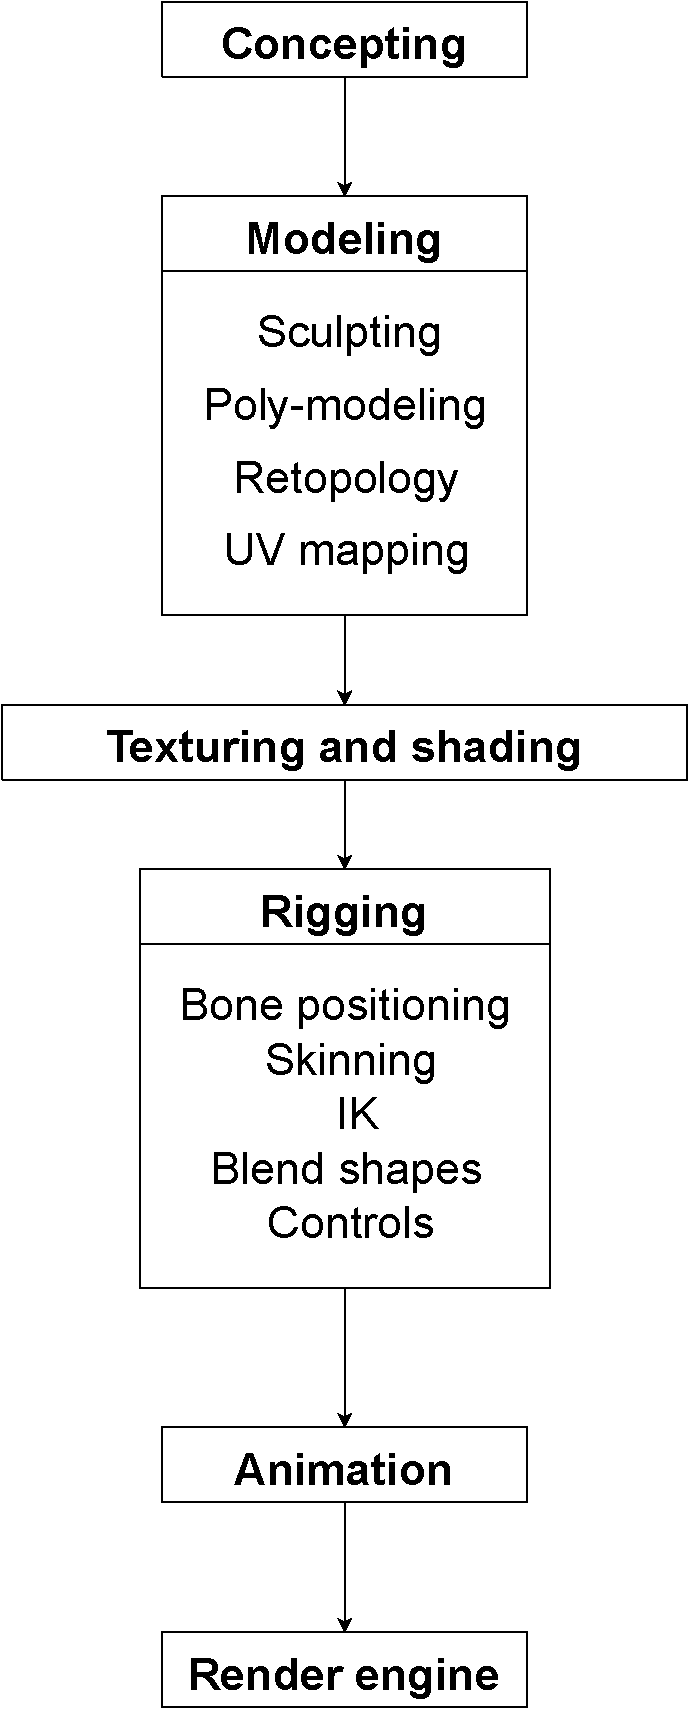
\includegraphics[width=30ex]{graphics/workflow_game.pdf}
    \caption{A typical video-game asset creation pipeline}
    \label{fig:assetCreationPipeline}
\end{figure}

\section{Concept art}
\label{sec:conceptArt}
Concept art is usually part of the pre-production of an asset. It is used to pre-visualise the idea and the mood of the game world.

A single concept is a drawing made by a specialised artist (called concept artist) and it is often achieved with digital painting. Other tools can be used to speed-up the workflow, like: photo-bashing, kit-bashing and using real-life pictures or 3D renders as a base to draw upon.

The final concept is then passed to a 3D modeler that has to make a mesh based upon the 2D drawing. For this reason, the reference drawing should require the modeler the minimum effort to translate it from 2D to 3D space (example of a final concept in figure \ref{fig:beetleCabConcept}).

\begin{figure}[hp]
    \centering
    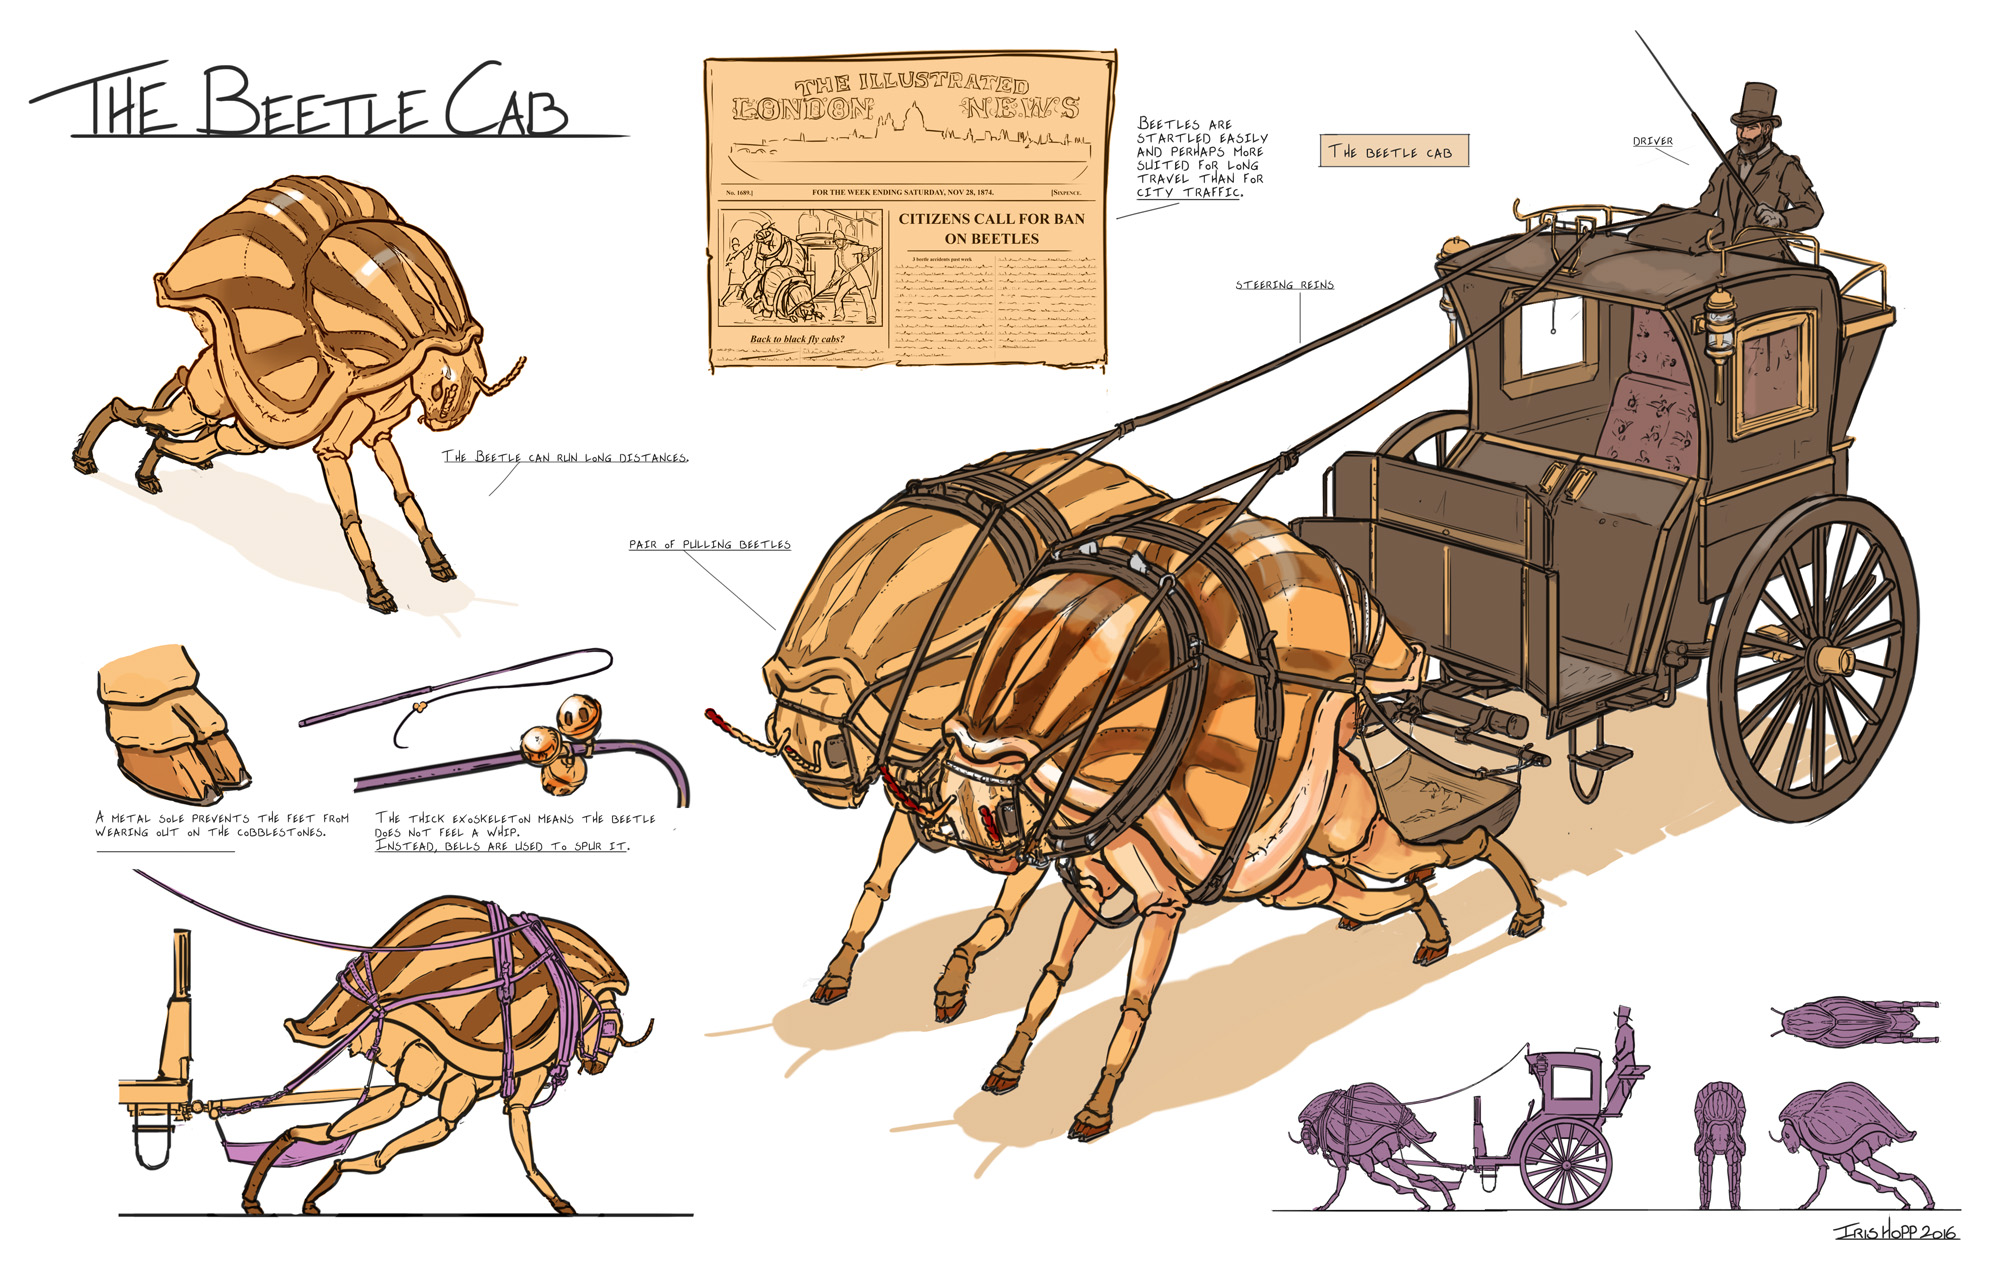
\includegraphics[width=\textwidth]{graphics/beetleCab_conceptArt.jpg}
    \caption[A final concept art of a fantasy carriage]{A final concept art of a fantasy carriage \\ \citeInFigure{Iris Hopp (Wikimedia Commons)} }
    \label{fig:beetleCabConcept}
\end{figure}

\section{Modeling}
\label{sec:modeling}
A 3D model is a set of vertices in 3D space that are connected to each other in order to generate the edges and the faces that shape an object. The mesh can be thought as a net that wraps the shape of the object, while topology determine how the vertices themselves are connected.

A mesh with few polygons is called low-poly and it is easy to edit by moving each single vertex individually (hence, low-poly modelling, Figure \ref{fig:polyModeling}). When a mesh has many polygons, it is called high-poly. A high-poly model is difficult to edit with low-poly modeling, unless using supporting tools or approaches like splines, modifiers or ``subdiv". On the other hand, it can be molded with digital brushes (process known as sculpting, Figure \ref{fig:sculpt}).

Hi-poly models, in turn, can be organic if the silhouette is mostly composed of soft edges (for example humans, animals and fabrics), and hard surface if the silhouette is mostly composed of hard edges (for example mechanical objects).

\begin{figure}[hp]
    \centering
    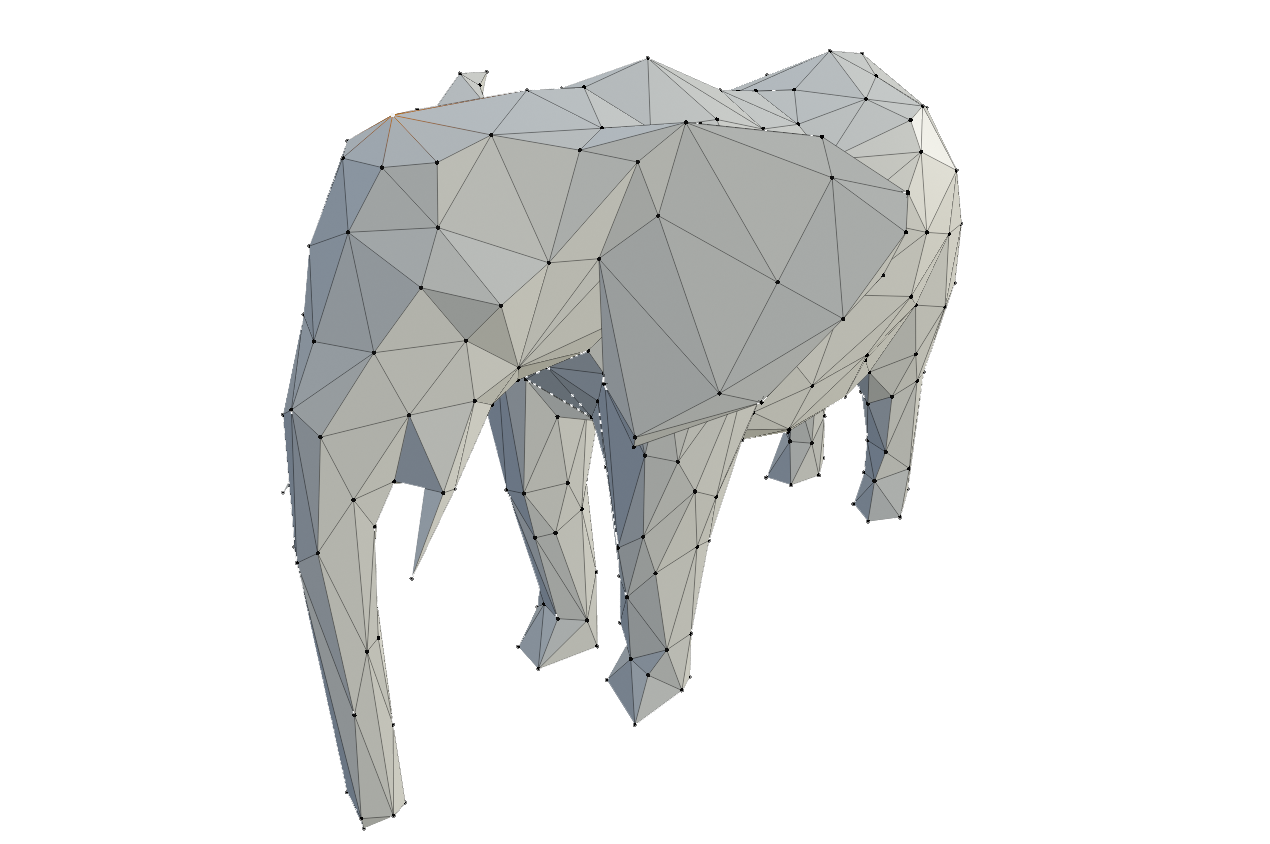
\includegraphics[width=45ex]{graphics/polyModeling_ex.png}
    \caption[Example of low-poly modeling]{Example of low-poly modeling \hspace{15ex} \\ \citeInFigure{ozgurcoteli (Turbosquid)} }
    
    \label{fig:polyModeling}
\end{figure}
\begin{figure}[hp]
    \centering
    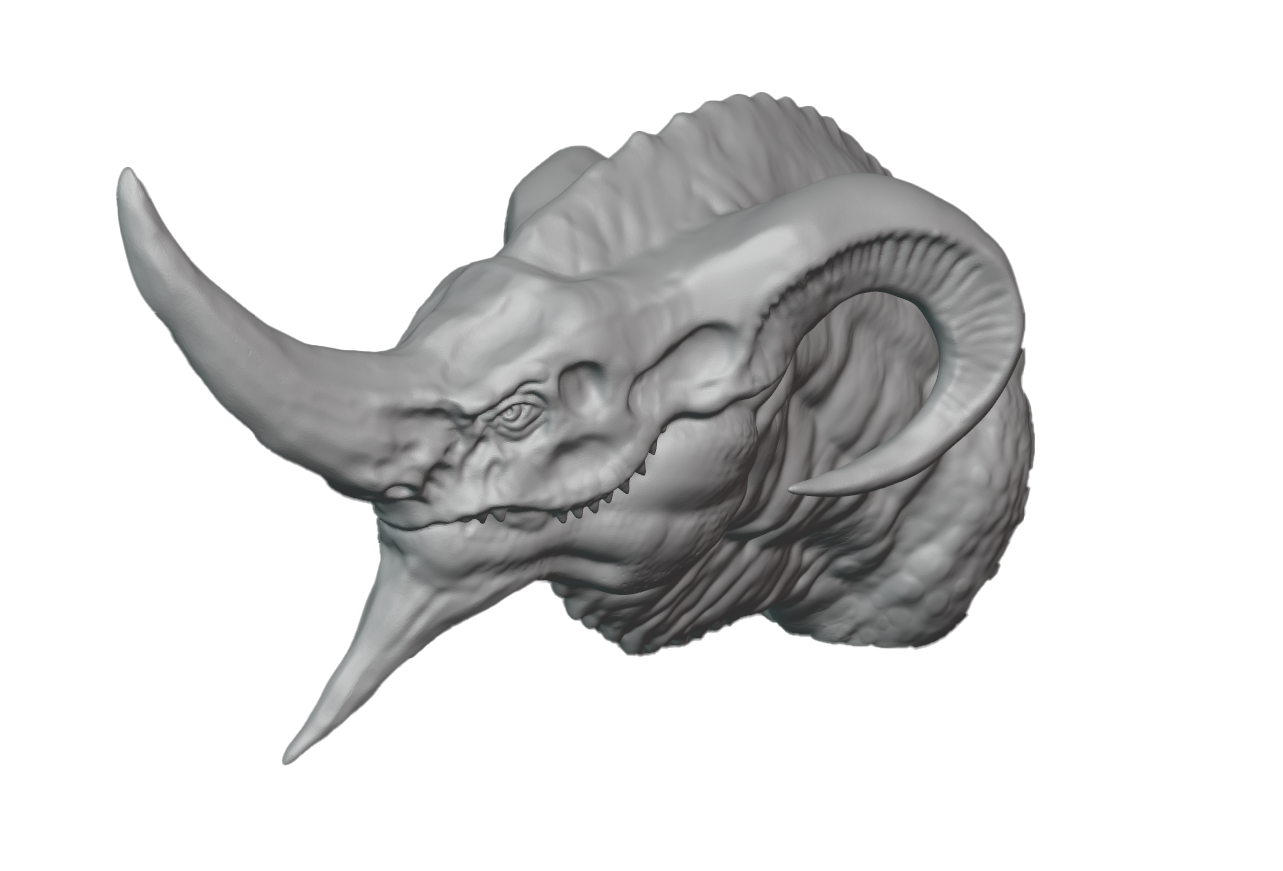
\includegraphics[width=45ex]{graphics/sculpt_ex.png}
    \caption[Example of a sculpted model]{Example of a sculpted model \hspace{15ex} \\ \citeInFigure{chauvanla (Turbosquid)} }
    \label{fig:sculpt}
\end{figure}

\subsection{Sculpting}
\label{subsec:sculpting}
Sculpting is a method to organically model a mesh like digital clay. In fact, the skill-set required in order to achieve professional results is similar to the one used by sculptors who employ traditional mediums.

An artist has at his disposal a set of brushes to alter the mesh displacement and connectivity. Altering mesh displacement is used to build or remove form to an object in order to get it to the desired shape, whereas altering the connectivity is used in order to increase or decrease the mesh density. Increasing the vertices' number is useful to get finer details in the sculpt where needed, while decreasing the number is useful to tune its broader shape (Figure \ref{fig:dyntopo}) (more details in section \ref{sec:sculptUI}).

\begin{figure}[hp]
    \centering
    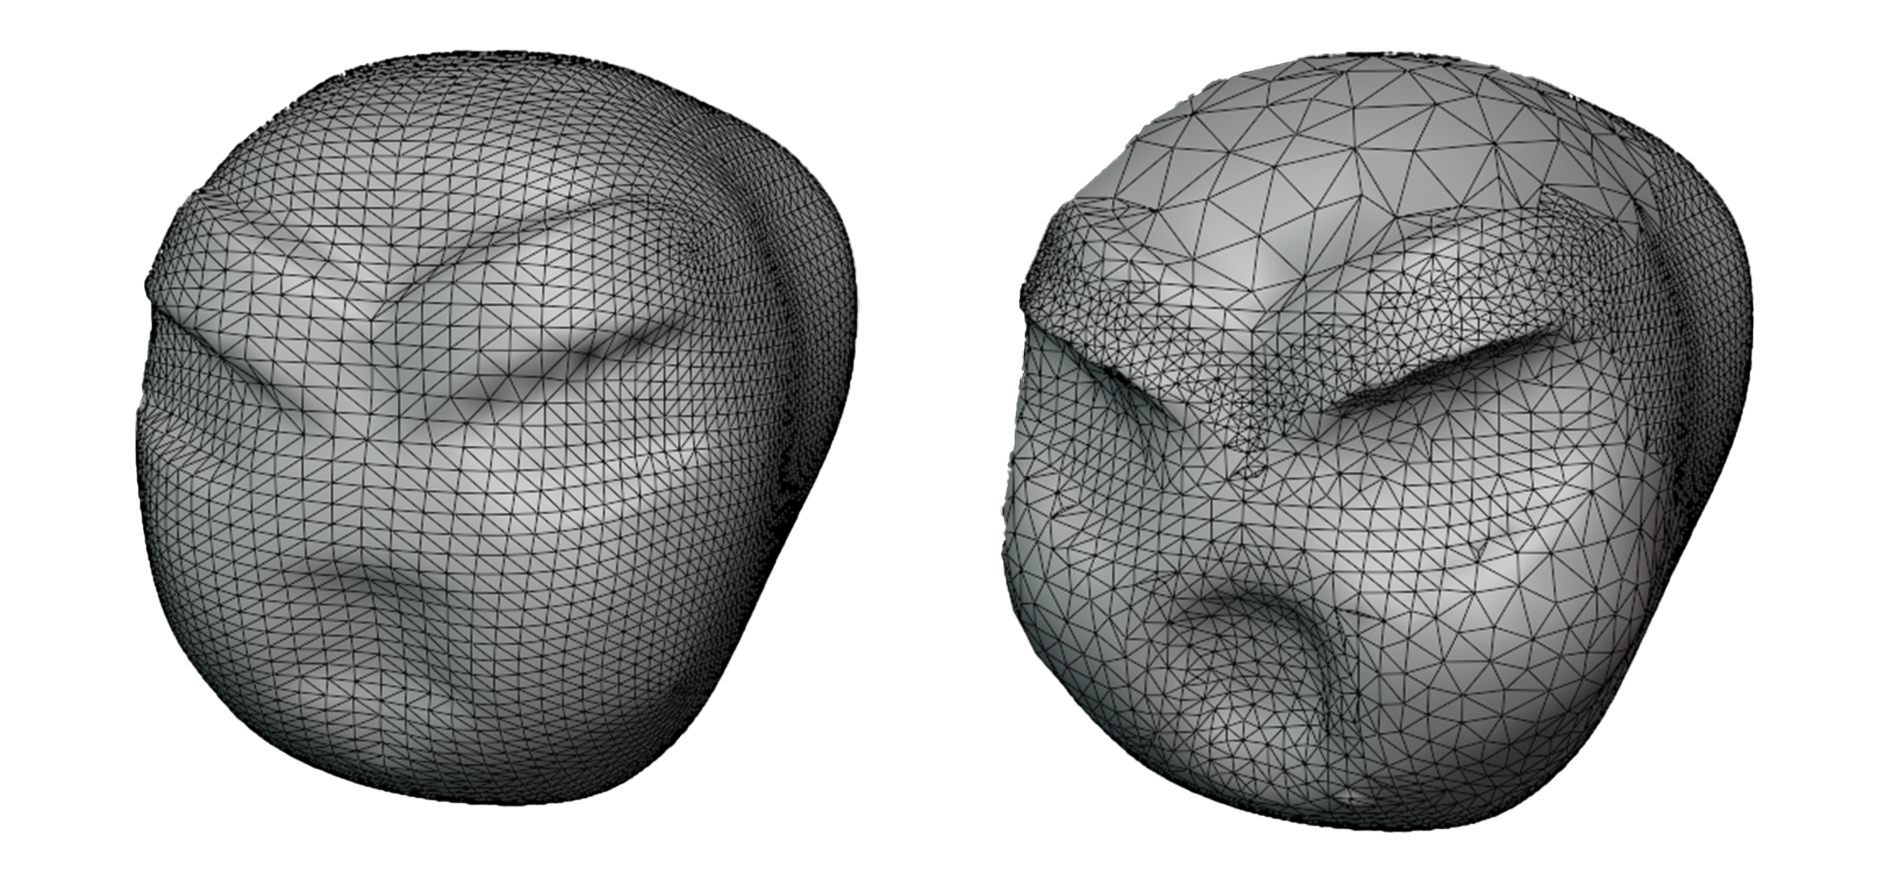
\includegraphics[width=56ex]{graphics/dyntopo_bfaft.png}
    \caption[Example of a model with dynamic adaptive resolution]{Example of a model with dynamic adaptive resolution (before/after)}
    \label{fig:dyntopo}
\end{figure}

\subsection{Making a pipeline-ready model}
\label{subsec:pipelineRdyModel}
The final steps of modeling are retopology and UV mapping.

Retopology is the action of re-making the model topology following some rules to optimise it for the pipeline. This implies that a finished model, depending on its destination, requires a certain type of topology. The ideal mesh is composed of quads, with edge loops that correctly follow its shape.

All the steps in the pipeline are optimised for quad-dominant topology. For example, game engines only use triangles, but the triangulation is implicit once the model is imported inside. UV maps, rigging and animation too are greatly favored by said topology.

Low-poly modeling allows an artist to control the shape of an object together with its topology. The resulting mesh is ready to proceed to the next steps.

Sculpting, on the other hand, in particular if using dynamic adaptive resolution, outputs a mesh with uneven topology (example of uneven topology in a character, Figure \ref{fig:bfRetopo}, later retopoligized, Figure \ref{fig:aftRetopo}). This implies that retopology is required.

UV maps are made to map a 2D picture (called texture) on the 3D shape (more details in section \ref{sec:texturingShading}). They are a 2D representation of the model's topology (an example on Figures \ref{fig:aftRetopo}, \ref{fig:chestUVtop} and \ref{fig:cleanTopology}).

\begin{figure}[hp]
    \centering
    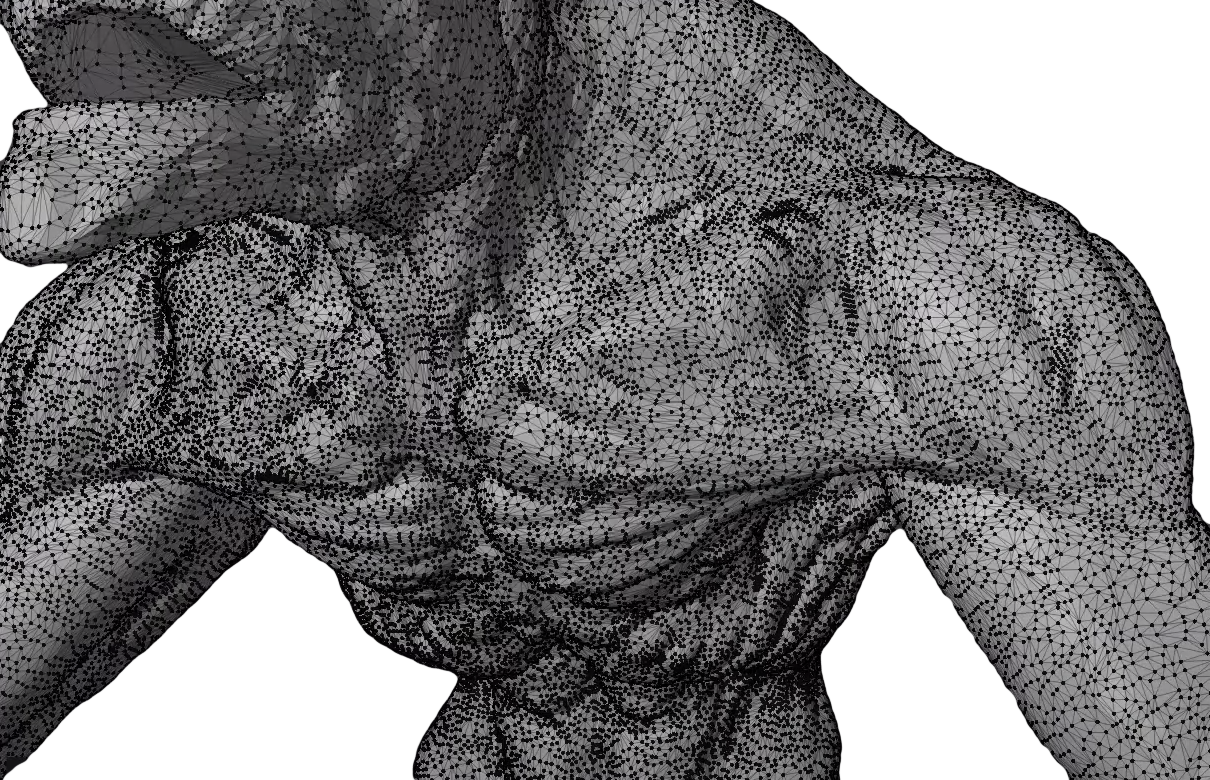
\includegraphics[width=45ex]{graphics/bfRetopo.png}
    \caption[Mesh with uneven topology]{Mesh with uneven topology (after sculpting) \hspace{15ex} \\ \citeInFigure{FlippedNormals} }
    \label{fig:bfRetopo}
\end{figure}

\begin{figure}[hp]
    \centering
    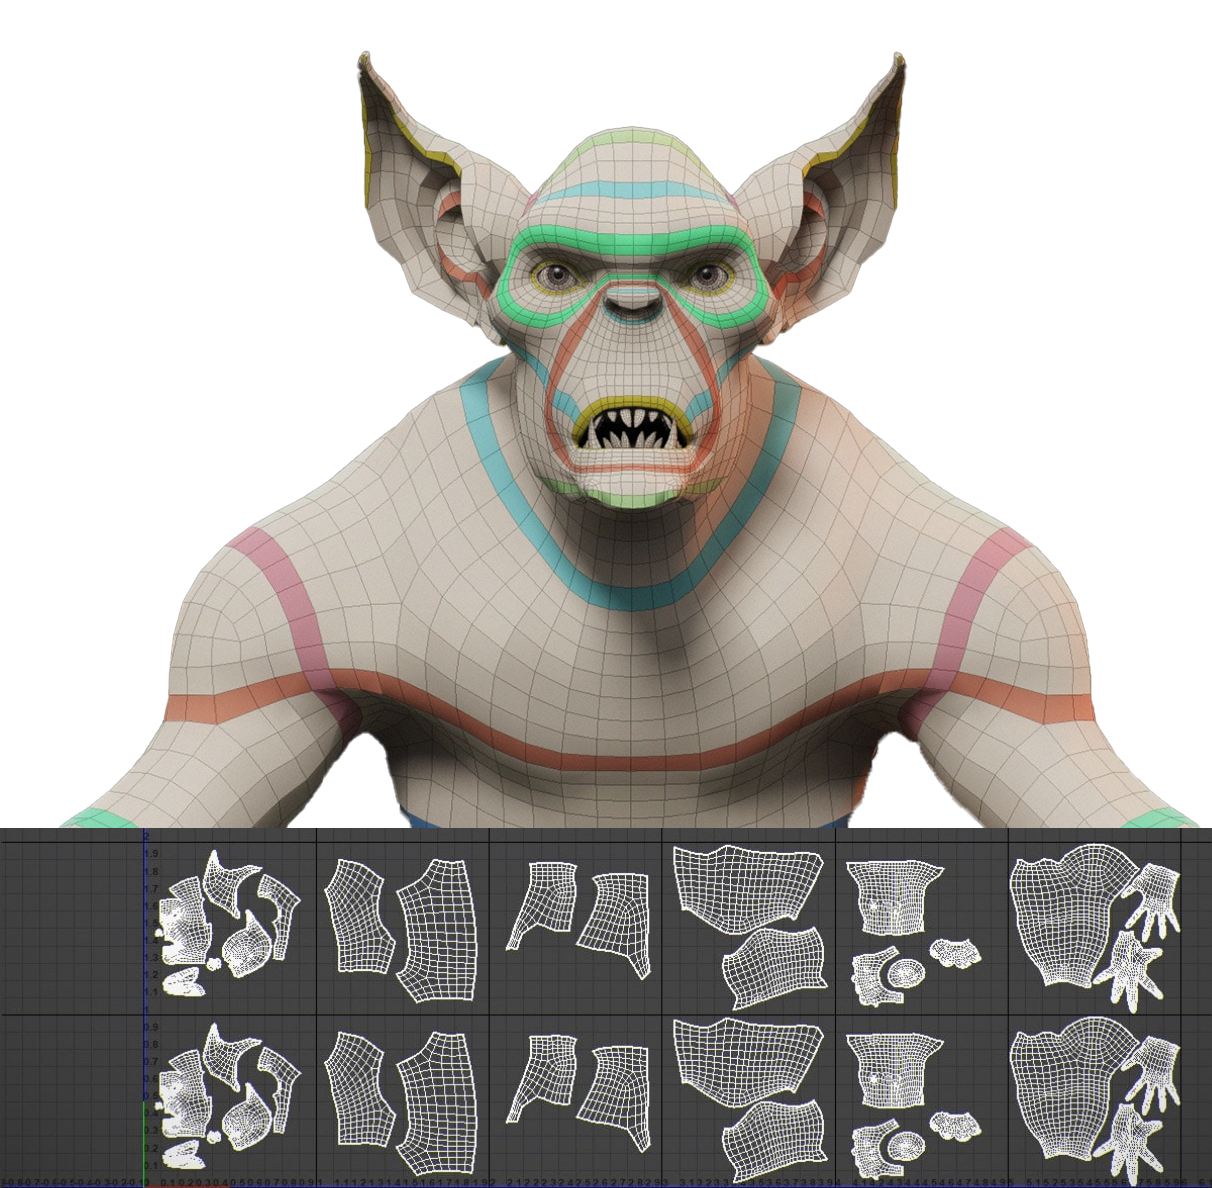
\includegraphics[width=45ex]{graphics/aftRetopo.png}
    \caption[Mesh with clean topology and UV-maps]{Mesh with clean topology and UV-maps \hspace{15ex} \\ \citeInFigure{FlippedNormals} }
    \label{fig:aftRetopo}
\end{figure}

\section{Texturing and Shading}
\label{sec:texturingShading}
A texture is a combination of texture elements (hence, texel or texture pixel). It is a digital image used to wrap a 3D model. They are usually a set of maps that are used to render the object.

The most common is the color map (or albedo) by which an artist paints or photo-stitches the color appearance of an object (Figure \ref{fig:chestTexture}). Other maps are then used depending on the needs.

\begin{figure}[hp]
    \centering
    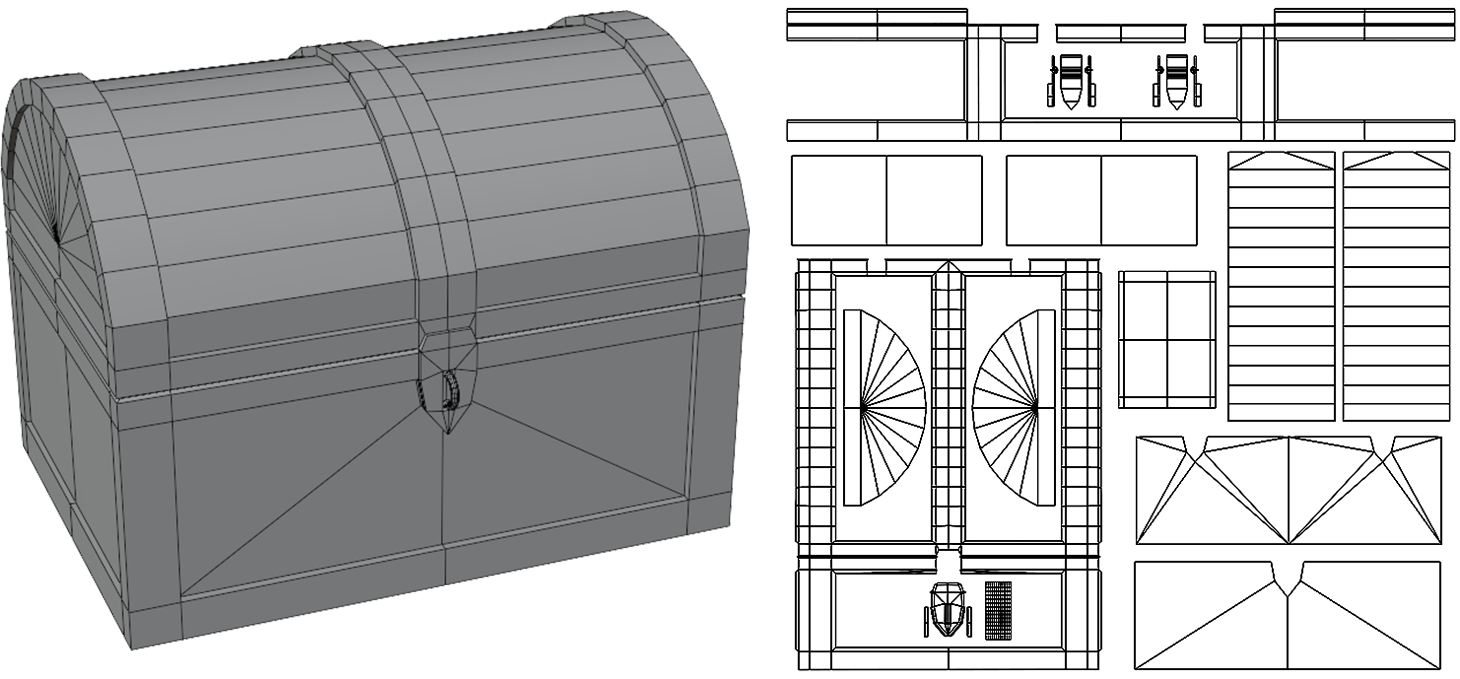
\includegraphics[height=25ex]{graphics/chest_UV_topology.png}
    \caption{A chest with topology and UV maps}
    \label{fig:chestUVtop}
\end{figure}

\begin{figure}[hp]
    \centering
    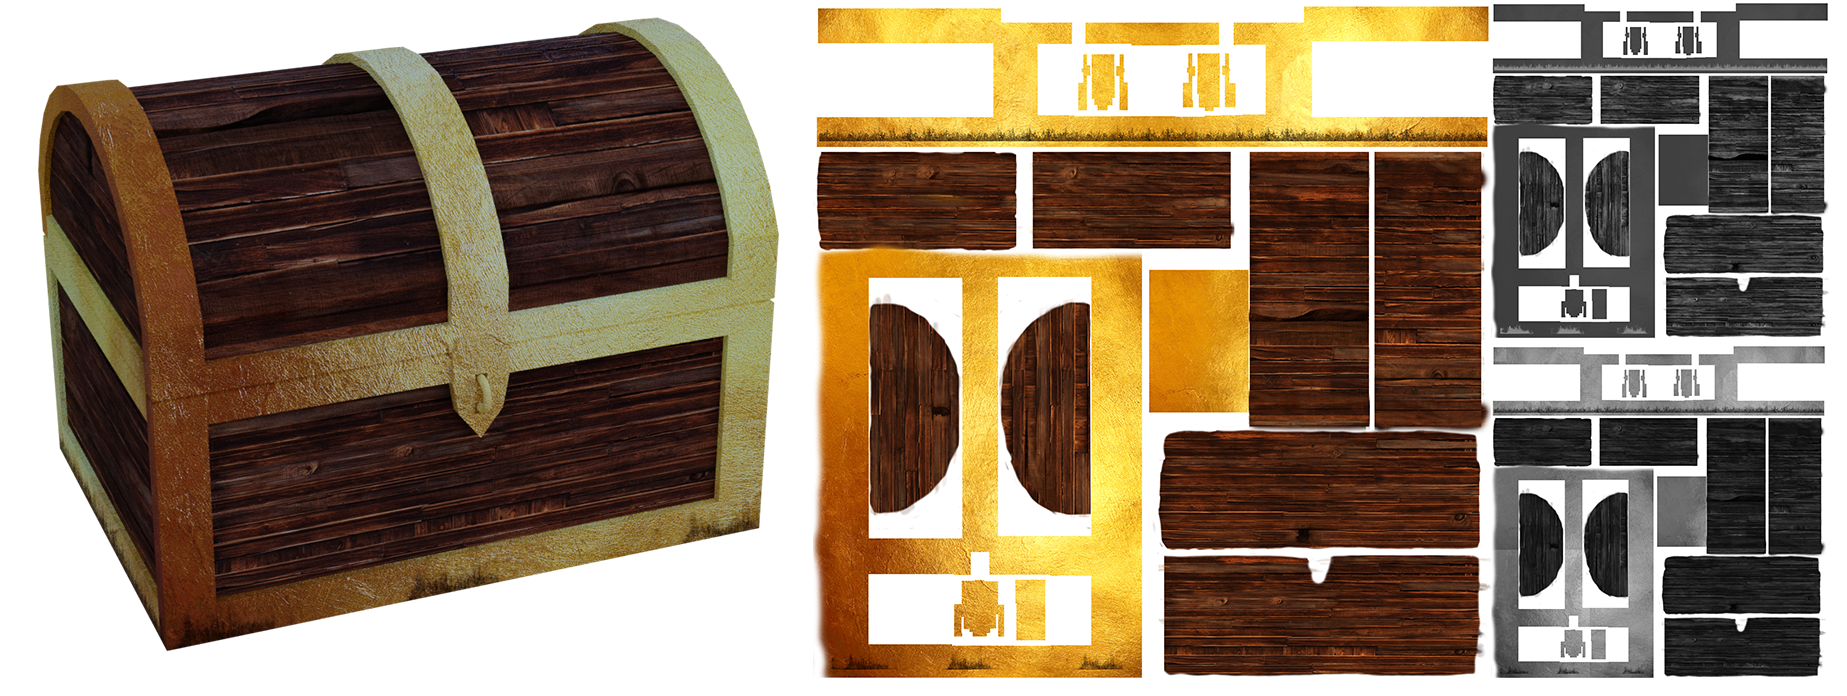
\includegraphics[height=25ex]{graphics/chest.png}
    \caption{The chest rendered with textures}
    \label{fig:chestTexture}
\end{figure}

Furthermore, a material, also known as shader, is added in order to decide how the model will interact with the light. It is composed of parameters that set the color, glossiness, transparency, luminosity, translucency of an object. Texture maps for a model are combined to one another, inside its shader before rendering. 

Shading information (computed during rendering) can be stored inside textures. This process is called baking; it optimises the calculations in expense of higher memory space.

\section{Rigging and animation}
\label{sec:riggingAnim}
Certain objects, for example characters, also need to be animated in order to have them move. In this case, the mesh needs to be rigged first. Rigging is the phase where the object's mesh is bound to a skeleton that drives its movement. The skeleton is composed of bones that affect the mesh vertices. Controls are then added to drive the skeleton and let the animator deform the object more easily (Figure \ref{fig:rain_rig}).

Mesh vertices are influenced by one or more bones to allow more organic deformations. Skinning is the action to create or modify these influences (called ``weights") in order to get to a desired deformation.

During the animation phase, an artist deforms the object in multiple poses that are then put accordingly in the timeline in order to give the illusion of movement. Each frame in the timeline which has an associated pose is called ``key-frame".

Inside games, unlike for films and TV, an animator creates many small animations that may be triggered in response to a player's command. All these small animations are later stitched together inside the game engine (section \ref{sec:gameEngine}).

\subsection{Skinning (editing of bone links)}
\label{subsec:skinning}
Skinning is part of the rigging phase, therefore it is a more technical process. A mesh in the rigging phase usually has already been modeled, so it has pipeline-ready topology (Figure \ref{fig:cleanTopology}) and UV maps. The topology from here-over should never be modified as it could compromise the rest of the pipeline.

During the rigging phase, a skeleton is created to decide how an object will deform. For a simple character, the bones that make up the skeleton are intuitively positioned at the human joints. Different or more complex models require positions based upon the required deformation.

The bones will move the vertices. Every bone affects a certain number of vertices; as such, every vertex is also affected by a certain number of bones.

A common skinning method used is LBS (linear blend skinning) \cite{tarini2014accurate}: it consists in giving a weight that corresponds to the influence a bone has on a vertex. Therefore, a vertex has $n$ weights corresponding to the number of bones that affect it. The sum of all the weights should be $1$, to allow the interpolation of every bone transformation. This results in clean deformations, with limitations \cite{lewis2000pose}, \cite{li2011automatic}.

\begin{figure}[hp]
\centering
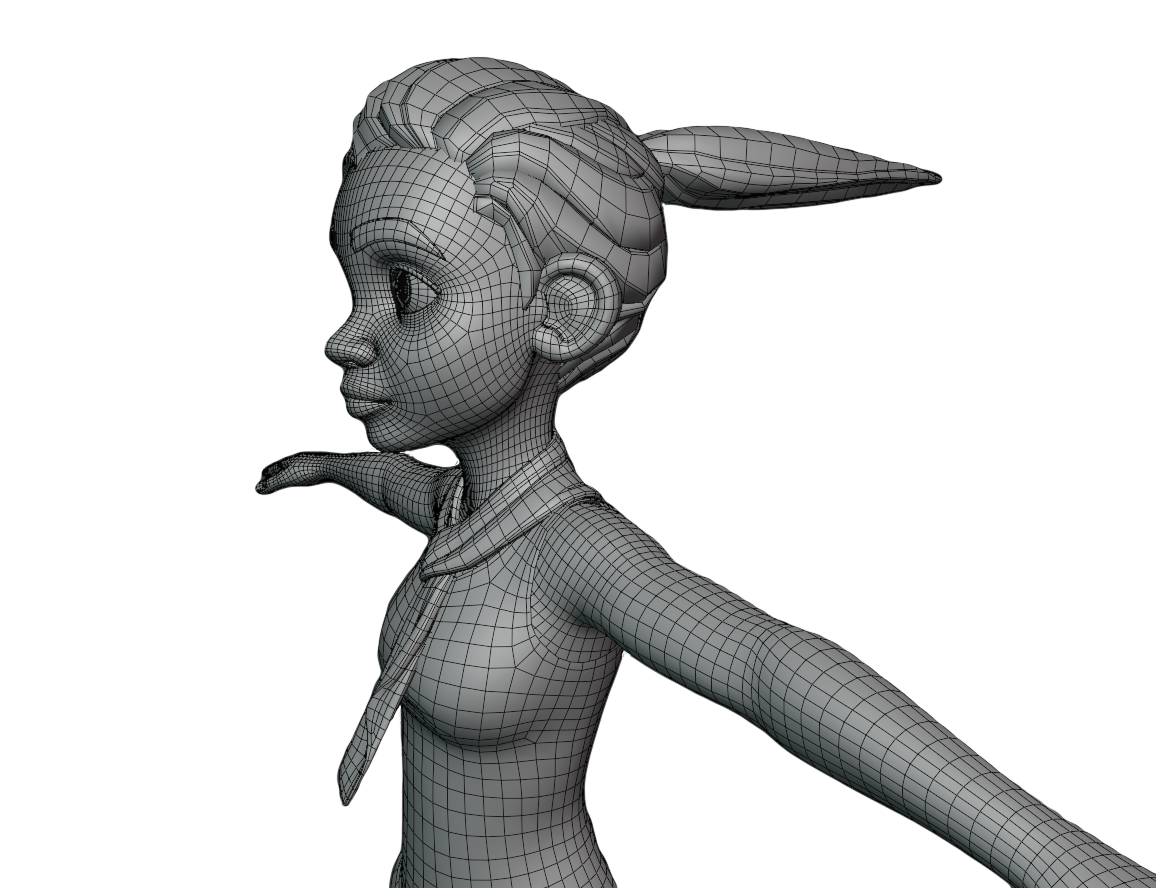
\includegraphics[width=45ex]{graphics/cleanTopology.png}
\caption[Example of a model with clean rigging-ready topology]{Example of a model with clean rigging-ready topology \\ \citeInFigure{Demeter Dzadik (Blender Cloud)} }
\label{fig:cleanTopology}
\end{figure}

\begin{figure}[hp]
\centering
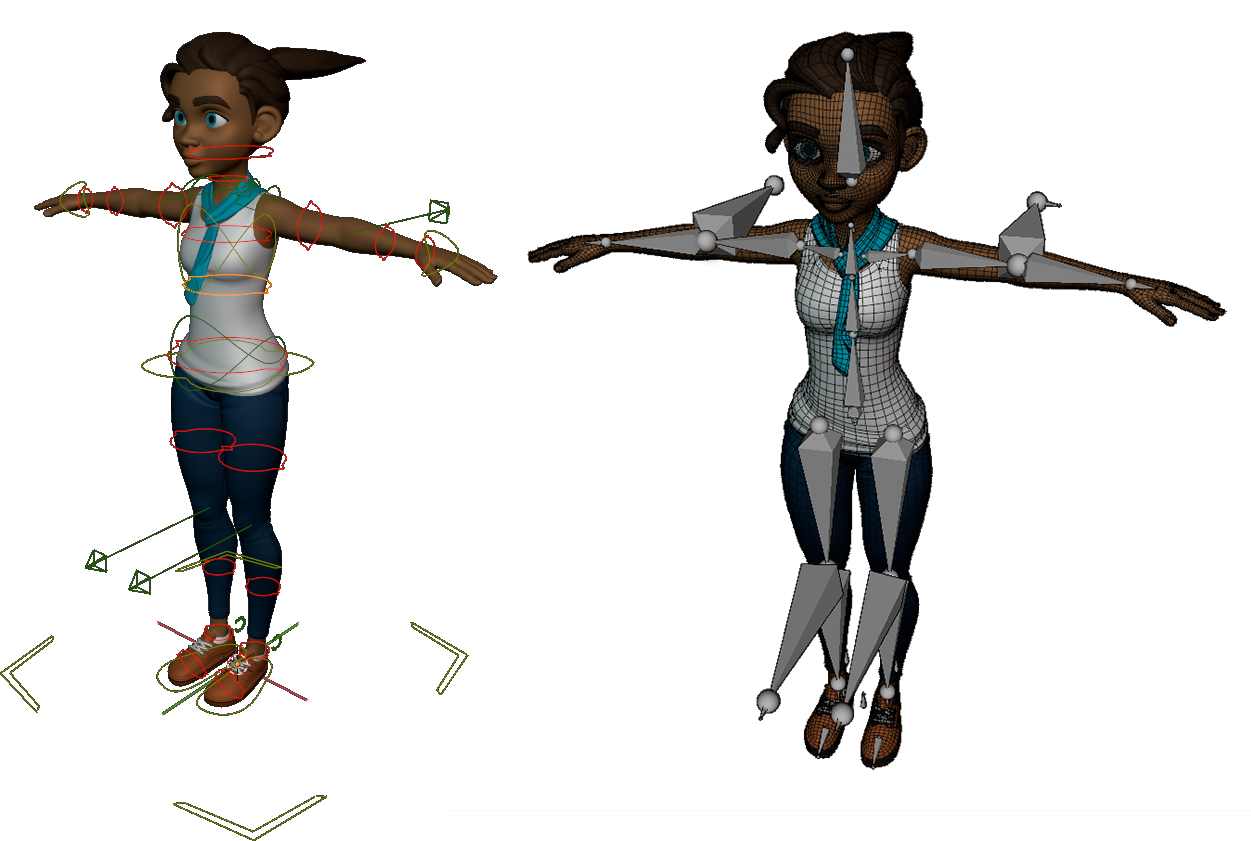
\includegraphics[width=65ex]{graphics/rain_rig.png}
\caption[The same model with controls and the skeleton that drives the motion]{The same model with controls (left) and the skeleton that drives the motion (right) \\ \citeInFigure{Demeter Dzadik (Blender Cloud)} }
\label{fig:rain_rig}
\end{figure}

In video-games, animated objects usually have vertices affected from two to a maximum of four bones.

\section{Game engine}
\label{sec:gameEngine}
Inside a game engine, each asset (2D and 3D assets, lighting and physics simulations, AI and audio) is combined in real-time. They must be merged by the game code in such a way as to create a seamless, interactive user experience. We can see how the assets produced in the pipeline on Figure \ref{fig:assetCreationPipeline} are kept separate, and stitched together inside the engine on Figure \ref{fig:gameEngineCombine}.

The animations are combined in a blend-tree where they do not have to just look good, but they also have to work alongside other data.

Moreover, game engines use real-time rendering that allows quick and smooth interaction that requires to render multiple frames every second (usually 30, 60 fps). However, obtaining physically accurate results is more complex. This is due to the algorithm involved, rasterisation (GPU-based), that doesn't try to replicate real life and, instead, requires more intervention to mimic the appearance of a scene. This is different from ray-tracing (CPU-based), used in off-line rendering for film and TV, that takes more time (seconds, minutes or hours, depending on the volume of the scene) in order to compute a single frame by approximating real-life light rays, although they are parallelizable on GPUs \cite{ludvigsen2010real}.

\begin{figure}[hp]
    \centering
    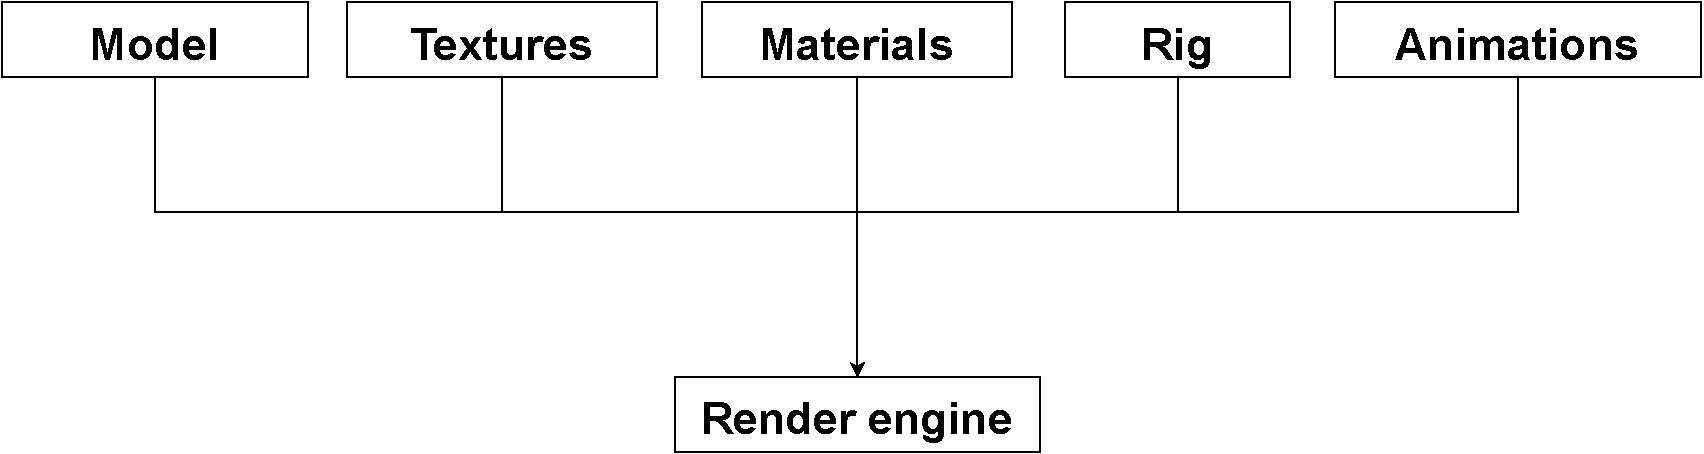
\includegraphics[width=\textwidth]{graphics/workflow_engine.pdf}
    \caption{Combining the object's assets inside a game engine}
    \label{fig:gameEngineCombine}
\end{figure}

\chapter{Background}
As we discussed on Chapter \ref{ch:intro}, we design a tool that lets a user edit skin weights by using a sculpting  interface. Internally, this tool solves an inverse problem: converting the 3D sculpts into skin.

In order to implement this idea, we will leverage on three existing software tools: classic skin weight editor (section \ref{sec:skinedit}), classic sculpting interfaces (section \ref{sec:sculptUI}), and standard numerical solvers (section \ref{sec:numsolv}). 

In this chapter, we shall discuss these three aspects of the work, that will be combined later in Chapter \ref{ch:implem}.

\section{Skin weight editor}
\label{sec:skinedit}
Authoring of skin weights is a technical skill of a digital artist (section \ref{sec:riggingAnim}). It is considered a challenging task to be done well and it requires a lot of trial and error to obtain good results, even for the more experienced artists \cite{li2011automatic}. This is due to the effects of the weights, i.e.\ their quality, that can only be evaluated by watching the deformations that they induce on each pose and animation. Observing only one pose is not enough to see the effect. The artist is also responsible of choosing the right weight amount to find the correct deformation. Vertices, in fact, often are very sensible to a slight change in influence.

Many 3D software suites used in the industry have tools to edit said weights (skin weight painting). Inside Maya and Blender, the artist paints the bones influences on the vertices, like colors. Usually, a color corresponds to a weight of 1, another to a weight of 0 and the in-betweens have colors to blend the the first two that correspond to more or less influence (figures \ref{fig:skinEditing_maya}, \ref{fig:skinEditing_blender}). The system has the option to ensure the normalisation of the weights, depending on the pipeline workflow.

\begin{figure}[hp]
    \centering
    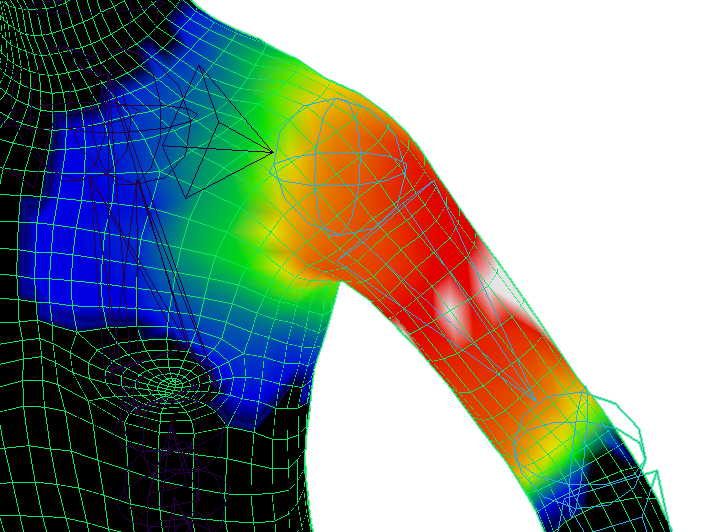
\includegraphics[width=35ex]{graphics/skinEditing_maya.png}
    \caption{Skin editing heat-map of a left shoulder joint inside Maya}
    \label{fig:skinEditing_maya}
\end{figure}

\begin{figure}[hp]
    \centering
    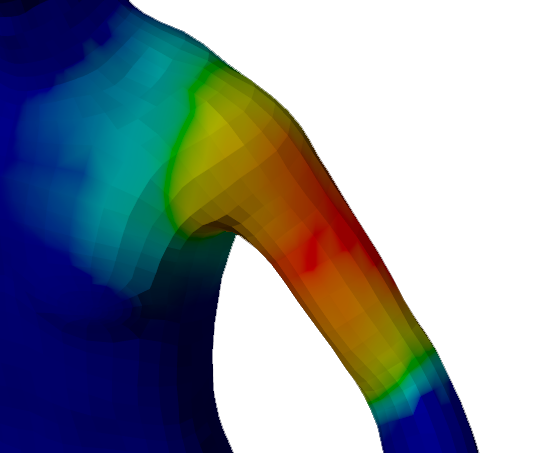
\includegraphics[width=35ex]{graphics/skinEditing_blender.png}
    \caption{Skin editing heat-map of a left shoulder joint inside Blender}
    \label{fig:skinEditing_blender}
\end{figure}

Automatic methods to calculate the weights are common: it is still an active research field. Researches mostly try to eliminate the process of manual skin authoring, or are focused on a specific area of anatomy \cite{lewis2000pose}.

Software suites, perhaps, offer simpler methods \cite{got2019developement}, generally used by an artist to have a base upon which edit. However, they usually do not reach a polished production-ready quality. As a consequence, manual authoring methods (like skin weight painting) still remain the most used, even though very time consuming.

The method we propose aims to simplify the assessment of any deformation by watching many poses, and to simplify the task of selecting the correct weights. As a result, it may require less trial and error.

\section{Sculpting interfaces}
\label{sec:sculptUI}
Sculpting, as we introduced in section \ref{subsec:sculpting}, is used to create static shapes geometry that will be animated in a separate step; so typical sculpting interfaces are different than our approach. Sculpting is very common, because it is intuitive for an artist, who has the illusion of manipulating plastic or clay material. He can also edit without worrying about technical details \cite{10.1145/2897824.2925956} like topology.

Usually the process \cite{spencer2010zbrush} can be broken down in: blocking phase, or low frequency details, where the artist shapes a relatively low-poly mesh to get the ``big forms" and proportions of an object; mid-frequency details, or secondary forms, where the object gets important landmarks: muscles, carvings. This is where a user starts to recognise the final result. In conclusion, we get high-frequency details, where the sculpt is finalised: this can include details like cloth texture or skin pores. Each phase is approximately associated to a level of details, or of subdivision. The more details are required, the more a mesh is subdivided, therefore has more polygons.

Many software suites adopt this editing mode. ZBrush, for example, is a program that focuses on sculpting (interface on figure \ref{fig:zbrushInterface}). It has become, as of 2020, the industry standard. It provides a very smooth interaction with the object and it can support, without hassles, a mesh with up to millions of polygons. It also provides a variety of brushes.

\begin{figure}[hb]
    \centering
    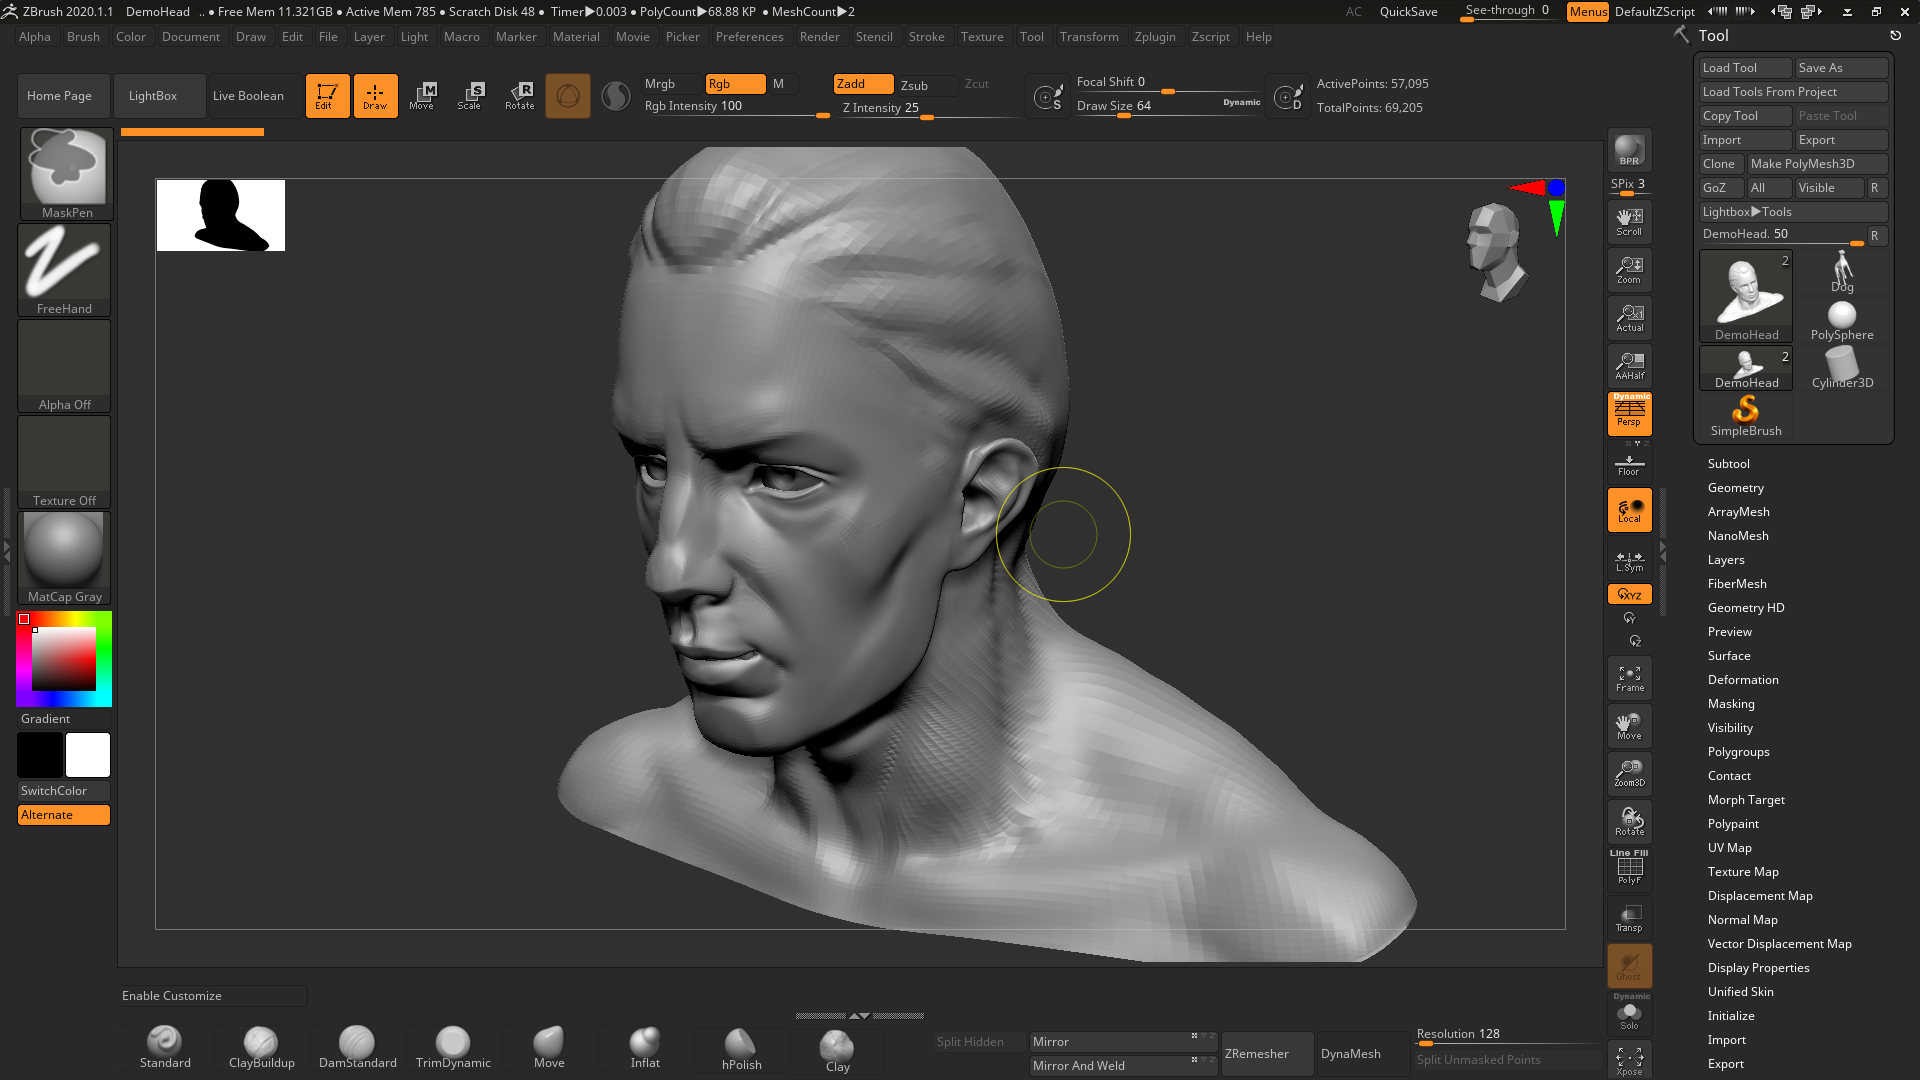
\includegraphics[width=59ex]{graphics/zbrushInterface.png}
    \caption{ZBrush interface}
    \label{fig:zbrushInterface}
\end{figure}

Blender also has a good sculpting mode (interface on figure \ref{fig:blender_sclupt_interface}). It has all the features described above, but lacks in supporting a very high polygon count. This can be expected by the fact that the program is general purpose (it is possible to complete every task in the pipeline) and open-source.

\begin{figure}[ht]
    \centering
    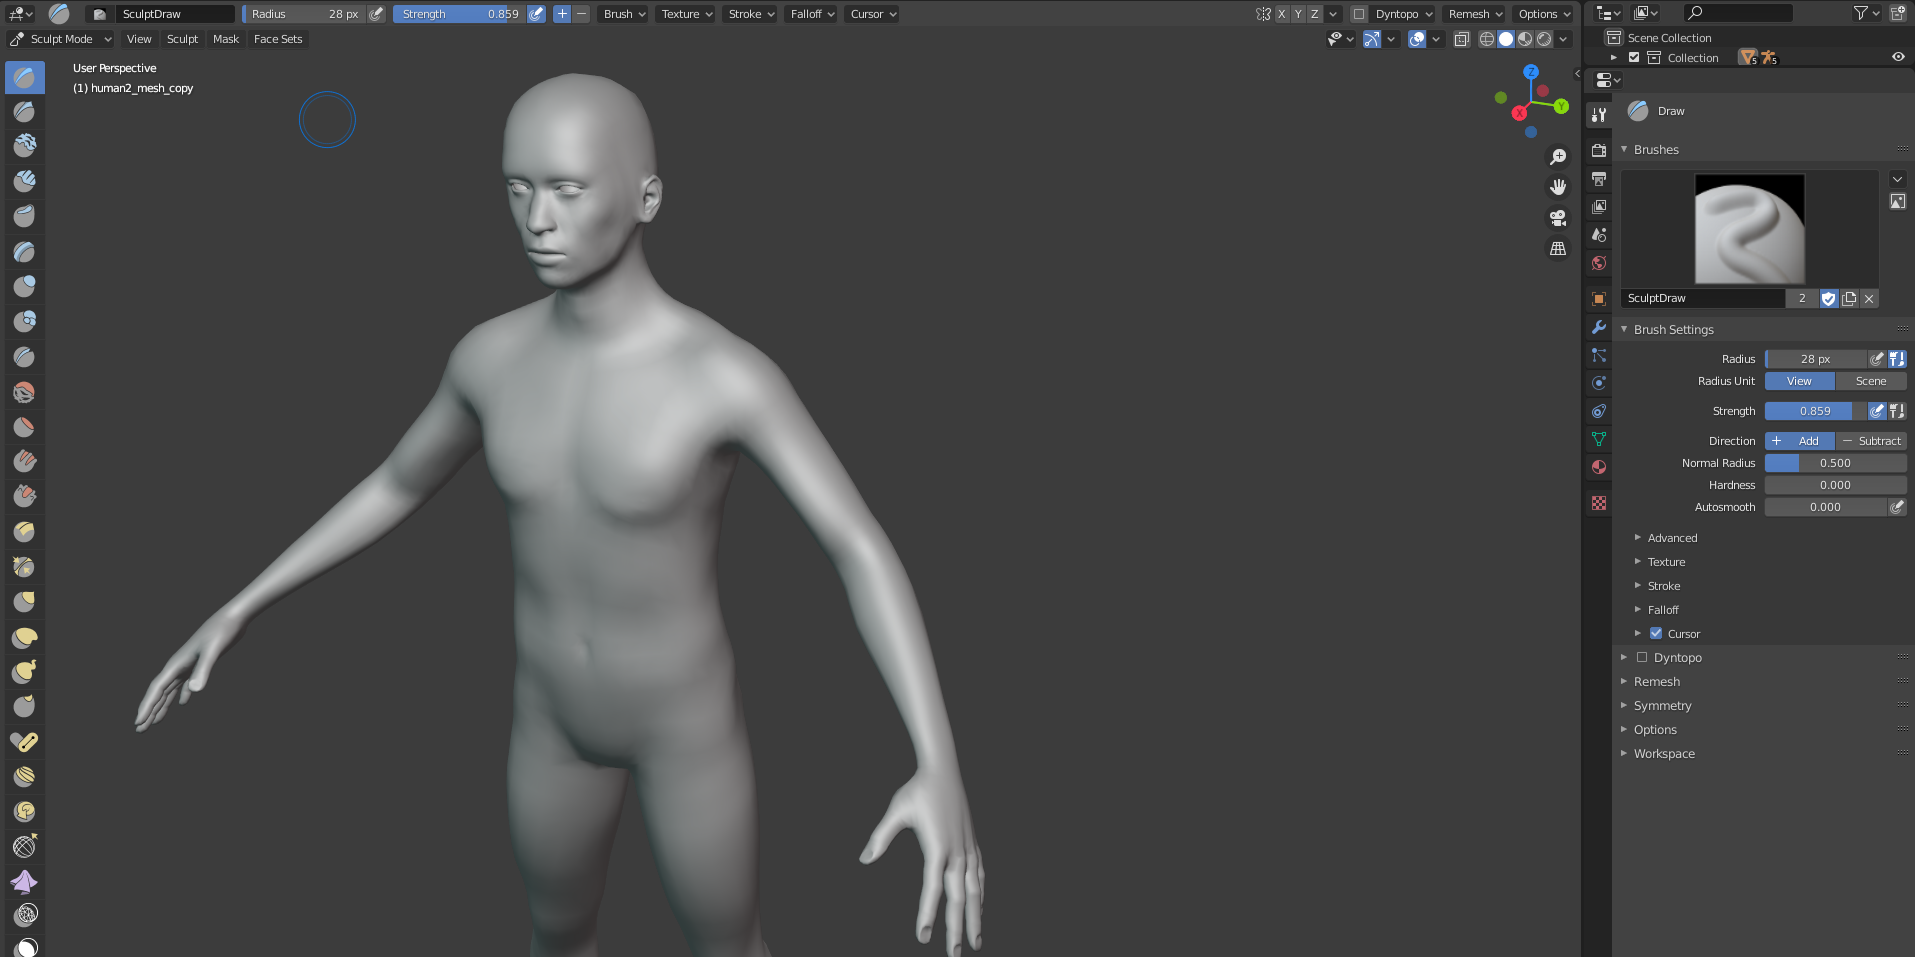
\includegraphics[width=60ex]{graphics/blender_sclupt_interface.png}
    \caption{Blender sculpting interface}
    \label{fig:blender_sclupt_interface}
\end{figure}

\section{Numerical solvers}
\label{sec:numsolv}
Our issue requires solving an inverse problem with systems of equations. In order to compute the solution, we use algorithms in numerical analysis. We can use linear least squares, or regularized least squares.

We list some notable applications intended for use with numerical analysis that may be useful for our purpose.

These are Python packages that are used for scientific computing: NumPy, SciPy, SymPy. The NumPy array is the basic data structure that many libraries understand and, together with SciPy, they provide extensive applications in numerical analysis; while SymPy is mostly used for symbolic manipulations. The Python tool stack does not attempt to replace the many critical codes and algorithms, but wraps them while providing rich data structures and programming paradigms \cite{perez2010python}.

Gurobi is a mathematical solver available for many modeling and programming languages.

Eigen is a C++ template library for linear algebra: matrices, vectors, numerical solvers, and related algorithms.

MATLAB is an environment for multi-paradigm programming language and numerical computing. It is very famous, because, as of 2020, it has more than 4 million users \cite{companyOverviewMathlab}.

Pardiso is a software for solving large sparse symmetric and unsymmetric linear systems of equations on shared-memory and distributed-memory multiprocessors.

\chapter{Objectives}
\label{ch:objectives}
We aim to build a new tool to author the mesh skinning information through sculpting. Converting the sculpting information to vertex weights essentially means transferring the position of a vertex: this consists in a transfer from the more intuitive information of a point in 3D-space ($xyz$) relative to its origin, to the one of a point that is not moved by a brush, but ``non-destructively" by a combination of weighted affine matrices (one per bone).

This means that, once we know the new displaced position of a vertex after a brush-stroke, we have to express it in terms of the weights that determine the transformation. The result should normally make the vertex deform in a position close to the one which has been displaced.

Every rigged model has a different number of bones that affects each vertex. In video-games, as we said in section \ref{subsec:skinning}, said number of bones is usually two or four. It is useful for us to have the highest possible degree of freedom, in order to get as close as possible to our objective. Consequently, we will assume that every vertex is affected by a number of four bones. We have to prepare the model for the conversion: in section \ref{sec:desparsificationMethod} we look for a solution.

Having four bones (so four weighted matrices) gives us a certain degree of freedom. However, we will have to deal with the known limitations of matrix interpolation in skeletal animation \cite{lewis2000pose}, that will probably be responsible for many converted vertices in a position far from the intended one.

\chapter{Analysis}

Now, we shall lay down the basic requirements for the software in order to support our script.

Then, we'll explain the paths to be explored before jumping to the conclusion of using Blender: either building a framework to develop the tool, or making a plug-in on an existing 3D software, in order to evaluate the applicability of our new method.

\section{Requirements}
\subsection{Import/export assets}

First, we need a software which can import and export a 3D asset in standard formats that supports mesh and animation data.

\subsection{GUI to sculpt and to visualize animation}
\label{sec:GUI_sclupt_anim_req}
The software for our research needs a 3D-view and a graphical user interface (GUI) to allow a model to be inspected. Then, it needs some features in order to be able to sculpt. We only need brushes that change the displacement of vertices, because it is not necessary to change the connectivity in any way, since the topology in the skinning phase has to remain the same, as we discussed earlier (section \ref{subsec:skinning}).

Moreover, the program must preview a skeletal animation. This means that we should be able to inspect an imported rigged character, which also has embedded poses.

Finally, we should be able to sculpt a model while it is already in a pose.

\subsection{Numerical optimiser}
In section \ref{sec:numsolv} we have listed certain software which might be useful to our project. Since we use Python scripting for Blender, it is natural to integrate it with NumPy and SciPy. However, they may be unnecessary: in fact, if we have a system with just three variables, inverting matrices should be sufficient (see section \ref{sec:skinSolvingMethod}).

\section{The alternatives}
Summarising the options: we either write a 3D software from scratch, or we look for the applicability of our new method on an already existing one.

\subsection{Starting from scratch}
\label{sec:framework_from_scratch}
In this first option, we can use C++ as the programming language, with Qt as the IDE; then the OpenGL library for rendering. We can also add Assimp library to handle the import and export of assets.

This would give us complete control over the new program and let us develop the research knowing all its parts. On the other hand, it would require to re-write software that is already in use in many 3D suites.

\subsection{Plug-in for an existing 3D-software}

In this second option, the path allows to immediately start focusing on an implementation. However, we should perform some tests in order to check if a program has all the requirements to further develop our ``animation sculpting" approach.

\subsubsection{Considered software alternatives}
It is possible to choose between many programs that can be scripted. We have considered the ones that are used more frequently in the industry, and are also common in freelance work. Therefore, we suppose they should have excellent support for scripting: Zbrush, Autodesk Maya and Blender. Now, let us analyse each of these three suites.

Zbrush has all the necessary features for sculpting, but doesn't support skeletal animations. It has Zscript as the internal language.

Autodesk Maya is an all-purpose 3D-program that has full support for animation, but does not have efficient sculpting tools. It supports Python and MEL (Maya Embedded Language) for scripting.

Blender is a free and open-source all-purpose 3D-software that supports both animation and sculpting. It provides an extensive Python library that accesses almost all the data structures inside. Also, the source code is available to be consulted and modified.

\subsubsection{Blender as a test framework}
Blender has all the requirements to directly evaluate the applicability of our approach:
\begin{itemize}
  \item Blender can import and export assets in common file formats;
  \item both animation and sculpting are well supported;
  \item we can import Python libraries, like NumPy, for numerical optimisation;
  \item the Blender Python API has a built-in operator to perform on mouse-up processing (section \ref{sec:on-mouse-up});
  \item it allows to access the source-code in order to perform changes to the program. This might be useful for our purposes.
\end{itemize}

In Chapter \ref{ch:method}, we are going to analyse the problem code-agnostic. In Chapter \ref{ch:implem} we'll implement the methods in Blender and we'll evaluate the results in order to see if the program is ready to further elaborate the research.

\chapter{Method}
\label{ch:method}

\section{Overview}
The user should be able to import a rigged model in the program, preview the model's poses and begin the sculpting session on a desired pose. Once the optimiser plug-in is run, skin weight desparsification (see section \ref{sec:desparsificationMethod}) is run once. The optimisation (section \ref{sec:skinSolvingMethod}) is computed after each brushstroke: this only happens for the vertices which changed their position. The user can edit as much as he needs. The resulting object can, in the end, be exported with the new weights.

\section{Computing while sculpting}

The conversion process (sculpting to weights) should be done ``on mouse-up", to remove the hassle of the wait of computing the conversion. This allows more forgiving computation time spans, which favors both the programmer and the artist.

In other words, when the user presses the left mouse button (or the surface with a pen tablet), every change on the mesh is registered as displacement, it is still common sculpting. As soon as the user releases the button, the conversion process begins, and it is possible to view the results immediately. The computation time should be forgiving enough to give the impression of real-time animation sculpting.

\section{Pre-processing: skin weight desparsification}
\label{sec:desparsificationMethod}
We assumed on Chapter \ref{ch:objectives} that every vertex in a mesh can be influenced by maximum four bones; as a consequence, we should write a program that  (no matter what rigged mesh has in input) produces a mesh which is ready for the next step, see section \ref{sec:skinSolvingMethod}.

In the original input, each vertex is linked to at most $K$ bones. Instead, we want to identify a set of exactly $N$ bones (four, in our case) that affect each vertex, by adding a small set of appropriate bones.

That is, we need to identify additional $N$-$K$ new bones for each vertex, which originally used to be linked to just $K$ bones. This will give more freedom to all subsequent optimizations of weights, without infringing the hard-coded constraints of computer animations used in games (see section \ref{subsec:skinning}). We call this process skin weight desparsification.

We select $N$-$K$ additional bones, looking for the ones that are close, in the skeleton hierarchy, to the already-used $K$ bounded: so, we use the notion of hop-distance in a graph. The new assigned bone weights will be initialised to $0$. The optimiser, in the next step, will be able to assign a weight $>0$ only to those new bones.

For more details on the implementation see section \ref{sec:desparsificationImplem}.

\section{Skin weight solving}
\label{sec:skinSolvingMethod}
We have 4 variables, one linearly dependent from the remaining three. Thus, we can solve the system with least squares (section \ref{subsec:leastsquaremodel}). After an in-depth analysis of the problem, it occurred that it can be divided in a series of little independent optimising problems, one per vertex (section \ref{subsec:regleastsqmmodel}); each of which can be expressed with least squares of only three variables.

As a result, it was possible to implement the solver ``manually" with a library that handles matrix inversion of dimension up to 4 (section \ref{sec:skinSolvingImplem}).

\subsection{Definitions}
Now, we have to define a nomenclature to illustrate the problem:\\ $A \in \{\mat{M}, \vect{v}, k\}$ can either be a matrix $\mat{M}$, a vector $\vect{v}$ or a scalar $k$.

In $A^c$, where $c \in \{r, p\}$, $r$ represents a position in rest pose and $p$ represents a position in a specific pose.

In $A_i$, where $i \in \mathbb{N}$, $i$ is the index of a mesh vertex. For example, $\vect{v}_i^c  = \{x, y, z\}$ is a generic vertex of a mesh, with $x, y, z \in \mathbb{R}$.

In $A[b_j]$, where $b, j \in \mathbb{N}$, $b$ is the index of a bone in a skeleton and $j$ is his subscript index since a bone index is sparse. For example $\mat{M}[1]_5$ means that the vertex $5$ is associated to the bone matrix $1$.

\subsection{Least squares method}
\label{subsec:leastsquaremodel}
Having $N$ vertices and $M$ bones in a mesh.

Knowing that we are in sculpt mode with our desired mesh selected. For each vertex $k \in \{0,\ \dots\ , N-1\}$ that has been displaced by a brush stroke, we do the following.

Having $\vect{v}_k^r$ the starting vertex position in a mesh in rest pose space and $\vect{t}_k^r$ the vertex in rest pose displaced after a brush stroke in sculpt mode. A vertex has $4$ starting weights $\{w[a_0], w[a_1], w[a_2], w[a_3]\}_k$, with $a \in \{0,\ \dots\ , M-1\}$ relative to $4$ rest pose bones matrices $\mat{M}[a_i]_k^r$ and $4$ pose-specific bone matrices $\mat{M}[a_i]_k^p$, with $i \in \{0,1,2,3\}$.

The matrix transformation for each bone is:

\[\mat{M}[a_i]_k = \mat{M}[a_i]_k^p (\mat{M}[a_i]_k^r)^{-1}\]

We can obtain the transformation matrix to take a vertex from rest-pose space to pose-specific space:

\[\mat{T}_k = \sum\limits_{i=0}^3 w[a_i] \mat{M}[a_i]_k\]

Now we can obtain the displaced vertex in pose-specific space:

\[\vect{t}_k^p = \mat{T}_k \vect{t}_k^r\]

The equation we are trying to solve, with $w[a_i]^f$ the final weights we are looking for:

\[\sum\limits_{i=0}^3 w[a_i]^f(\mat{M}[a_i]_k \vect{v}_k^r) = \vect{t}_k^p\]

By setting $\vect{d}_i = \mat{M}[a_i]_k \vect{v}_k^r$ and knowing that $w[a_3]=1 - (w[a_0] + w[a_1] + w[a_2])$, we get:

\[w_0^f(\vect{d}_0-\vect{d}_3) + w_1^f(\vect{d}_1-\vect{d}_3) + w_2^f(\vect{d}_2-\vect{d}_3) = \vect{t}^p - \vect{d}_3\]

We can order the equation as matrices:

\begin{equation*}
\mat{D}=
\begin{bmatrix} 
(\vect{d}_0-\vect{d}_3)_x & (\vect{d}_1-\vect{d}_3)_x & (\vect{d}_2-\vect{d}_3)_x \\
(\vect{d}_0-\vect{d}_3)_y & (\vect{d}_1-\vect{d}_3)_y & (\vect{d}_2-\vect{d}_3)_y \\
(\vect{d}_0-\vect{d}_3)_z & (\vect{d}_1-\vect{d}_3)_z & (\vect{d}_2-\vect{d}_3)_z
\end{bmatrix}
\quad
\vect{w} =
\begin{bmatrix}
w[a_0]^f & w[a_1]^f & w[a_2]^f
\end{bmatrix}
\end{equation*}

so

\[\vect{w}=\mat{D}^{-1}(V_t-d_3)\]

And the final weights should be:

\[\vect{w}_k^f = \{w[a_0]^f, w[a_1]^f, w[a_2]^f, w[a_3]^f\}\]

with

\[w[a_3]^f=1 - (w[a_0]^f + w[a_1]^f + w[a_2]^f)\]

\subsection{Regularised least squares method}
\label{subsec:regleastsqmmodel}
The approach in section \ref{subsec:leastsquaremodel} does not work on its own, because we cannot infer a position by finding the minimiser based just upon the target position. As a result, the system is ill-posed, therefore it is impossible to fit and most of the matrices we construct do not have an inverse.

We have to take into consideration the starting weights (or old weights) of each vertex, in order to tell the system that the ``new" weights we are looking for should tend to the initial state. In this way we obtain a RLS system that allows the introduction of further constraints that uniquely determine the solution.

By having:

\begin{equation}
    \label{eq:matrixInterp}
    \mat{A}\vect{w}=\vect{b}
\end{equation}

as the generalised equation. $\mat{A}$ is a 3x3 matrix, $\vect{b}$ is the 3D column vector of the known terms and $\vect{w}$ is the column vector of the three independent variables. We want to find:

\[\min\vect{w} \|\mat{A}\vect{w}-\vect{b}\|^2 \Rightarrow f'(\vect{w}) = 0\]

\[f(\vect{w}) = \|\mat{A}\vect{w}-\vect{b}\|^2 = \vect{w}^T\mat{A}^T\mat{A}\vect{w} - 2\vect{w}^T\mat{A}^T\vect{b} + \vect{b}^T\vect{b}\]

\[f'(\vect{w}) = 2\mat{A}^T\mat{A}\vect{w} - 2\mat{A}^T\vect{b}\]

\[f'(\vect{w}) = 0 \Rightarrow 2\mat{A}^T\mat{A}\vect{w} = 2\mat{A}^T\vect{b}\]

\[\mat{A}\vect{w} = \vect{b}\]

\[\min\vect{w} = \mat{A}^{-1}\vect{b}\]

Setting $\vect{b}' = -2\vect{b}$

\[\min\vect{w} = -\frac{1}{2}\mat{A}^{-1}\vect{b}'\]



This is possible, for our problem, only by using RLS on equation \ref{eq:matrixInterp}. This means we have to compose multiple Quadratics in order to obtain the final system.

The first one is, seen previously in section \ref{subsec:leastsquaremodel}:

%FIRST QUADRATIC
\[\|\mat{D}\vect{w}-\vect{p}\|{^2} = \vect{w}^T \mat{D}^T\mat{D}\vect{w} - 2\vect{w}^T\mat{D}^T \vect{p} + \vect{p}^T\vect{p}\]

where $\vect{p}=\vect{t}^p - \vect{d}_3$.

Having the starting, known, weights for a vertex:

\[\vect{o}_k = \{o[a_0], o[a_1], o[a_2], o[a_3]\}\]

We construct the second Quadratic that regularises the new weights based upon the first three starting ones. The parameter $k$ will control the power of the regularisation, therefore also the invertibility of the matrix.

\[\vect{o}^{3d} = \{o[a_0], o[a_1], o[a_2]\}\]
%SECOND QUADRATIC
\[\|k\mat{I}\vect{w}-k\vect{o}^{3d}\|^2 = \vect{w}^T (k^2\mat{I}) \vect{w} - 2 \vect{w}^T k^2(\vect{o}^{3d})^T + k^2 (\vect{o}^{3d})^T\vect{o}^{3d}\]

We now construct the third Quadratic that regularises the new weights based upon the fourth weight $o[a_3]$.

Having $\mat{J}_3$ a $3x3$ Matrix of all ones and $\vect{j} = \mat{J}_{3,1}$ a column Vector of all ones.

%THIRD QUADRATIC
\[\|k\mat{J}_3\vect{w}-k(o[a_3]\vect{j} - \vect{j})\|^2 = \vect{w}^T (k^2\mat{J}_3) \vect{w} + 2 \vect{w}^T k^2(o[a_3]\vect{j} - \vect{j}) + k^2(o[a_3]-1)^2\]

We can now sum all three elements to arrive to:

\[\mat{A} = \mat{D}^T\mat{D} + k^2\mat{I} + k^2\mat{J}_3\]
\[\vect{b}' = -2\mat{D}^T \vect{p} - 2k^2(\vect{o}^{3d})^T + 2k^2(o[a_3]\vect{j} - \vect{j})\]
\[c = \vect{p}^T\vect{p} + k^2(\vect{o}^{3d})^T\vect{o}^{3d} + k^2(o[a_3]-1)^2\]

So the final Quadratic will be:

\begin{equation}
\label{eq:evaluateQuadratic}
\vect{w}^T\mat{A}\vect{w} + \vect{b}'\vect{w}^T + c
\end{equation}

And the minimiser:

\[\vect{w}^{min}_k = \min\vect{w} = -\frac{1}{2} \mat{A}^{-1}\vect{b}'\]

\subsection{Normalising}
\label{sec:normalise_method}
Our linear system does not have a weight boundary between 0 and 1. Our implementation in Blender requires this limitation. Since we are solving the system manually, and not by using dedicated libraries, we need to impose it.

We make a new Quadratic that will then be added to the previous system only if a specific weight value in the vector of minimisers is negative.

$\vect{w}^{min}_k$ is made of each component of the vector of minimisers also with the linearly dependent fourth component:

\[\vect{w}^{4d}_k = \{w[a_0], w[a_1], w[a_2], w[a_3]\}\]

We set $h$ as the parameter that controls the power of the normalisation.

\begin{equation*}
\mat{M_x}=
    \begin{bmatrix}
    h & 0 & 0 \\
    0 & 0 & 0 \\
    0 & 0 & 0
    \end{bmatrix}
\quad
\mat{M_y}=
    \begin{bmatrix}
    0 & 0 & 0 \\
    0 & h & 0 \\
    0 & 0 & 0
    \end{bmatrix}
\quad
\mat{M_z}=
    \begin{bmatrix}
    0 & 0 & 0 \\
    0 & 0 & 0 \\
    0 & 0 & h
    \end{bmatrix}
\end{equation*}

The new matrix is added to the $\mat{A}$ in formula (\ref{eq:evaluateQuadratic}) based upon which element of the vector is negative.

The fourth weight is different from the other three: the new Quadratic is still added to the system only if $w[a_3]$ is negative.

\[\vect{l}=\{-2, -2, -2\}\]

\[\vect{w}^T (\mat{A} + h\mat{J}_3) \vect{w} + (\vect{b}' + h\vect{l}) \vect{w}^T + hc
\]

The minimiser of the new Quadratic should ensure that the boundary $[0, 1]$ is respected.

In conclusion, in order to remove any fluctuations in machine error, we apply a crude algorithm to normalise the vectors. This algorithm takes a vector, sums each element to the opposite its minimum and then divides it to its maximum. This happens only if the minimum is negative, or the maximum is $>1$. More on the implementation Chapter (section \ref{sec:normalise_implem}).

This approach, for now, does not produce good results. We can see the effects of the normalisation on a model in section \ref{sec:skinweightsolving_results}.

\chapter{Implementation}
\label{ch:implem}

\section{Basics of scripting in Blender}

We can access every aspect of the program with Blender's own API (Application Programming Interface) called bpy (Blender Python).

\begin{lstlisting}
import bpy
\end{lstlisting}

Other libraries will be used, but they will be specified later when necessary.

We now need a way to access information about: the mesh (vertices, edges, faces), the rig (skeleton, bones, rest-pose, any other pose) and the skinning (weights per vertex and referred bone). The skeleton in Blender is called armature.

In order to obtain the object data, there first has to be a reference from the members available in the context: the area of Blender which is currently being accessed.

\begin{lstlisting}
object = bpy.context.active_object
\end{lstlisting}

Once we get the correct reference, we can access its data:

\begin{lstlisting}
object_data = object.data
vertices = object_data.vertices

for vertex in vertices:
    print("Coordinates xyz of a single vertex:", vertex.co)
\end{lstlisting}

The same can be performed for any other data structure, with a few exceptions. We will specify them later when needed.

In addition, we use two libraries in order to facilitate our calculation. One is NumPy (section \ref{sec:numsolv}) and the other is Mathutils, a library used in Blender \cite{BlenderAPI} to manage Vectors and Matrices.

\begin{lstlisting}
import numpy as np
import mathutils
\end{lstlisting}

\section{Blender Modal Operator}

Operators are a way to implement a Python script into Blender \cite{BlenderAPI}.

The modal operator is crucial to achieve on mouse-up processing, as it is fundamentally built to perform actions while other Blender functions are running; and it does not freeze the interface during a script computation.

We shall take a look at its main structure.

\subsection{Inside a Class}

Every new operator in Blender inherits from the Class Operator.

\begin{lstlisting}
class SimpleModalOperator(bpy.types.Operator):
    def execute(self, context):
    def invoke(self, context, event):
    def modal(self, context, event):
\end{lstlisting}

The execute function is the simplest way to run commands without the user input. It also allows the operation to be repeated from a macro or another script.

The invoke function is used at the moment the operator is called, to initialize it from the current context. It is typically used to assign properties which are later used by other functions.

The modal function is the core of the class, as it will keep being run to handle events until it returns ``FINISHED" or ``CANCELLED". Every time a new event is detected, such as a mouse click or key press, the function will be called.

\subsection{Setting initial parameters}

Inside the invoke method, we can specify initial parameters that than can be used inside the modal method to be processed.

\begin{lstlisting}
def invoke(self, context, event):
    #some useful functions...
    
    #add the modal operator to the window manager (handles open windows and other user interface data)
    context.window_manager.modal_handler_add(self)
    
    #the operator does not exit immediately after invoke finishes:
    return {'RUNNING_MODAL'}
\end{lstlisting}

Inside the modal method we can detect the user actions and determine when the user presses and releases the left mouse button.

\begin{lstlisting}
def modal(self, context, event):
    if event.type=='LEFTMOUSE' and event.value=='PRESS':
        self.mousePressed = True
        #instructions to perform when the left mouse button is pressed

    if event.value == 'RELEASE' and self.mousePressed:
        self.mousePressed = False
        #instructions to perform when the left mouse button is released
\end{lstlisting}

Sometimes, the event value ``RELEASE" pops-up twice after the mouse button is physically released, so it is necessary to use a Boolean variable to check if the mouse is already pressed.

\section{Testing on mouse-up processing}
\label{sec:on-mouse-up}
We write a simple program that averages the distance between the position of a vertex, before and after being edited. This is a test to evaluate the ability to process the mesh after each brush-stroke. It is also useful to check where the mesh is being edited and apply a function only to those specific vertices.

\begin{lstlisting}
#inside the modal method
if event.type == 'LEFTMOUSE' and event.value == 'PRESS':
    self.mousePressed= True
    
    #get all vertex positions
    for v in bpy.context.active_object.data.vertices:
        #startingVerts is a class variable list 
        self.startingVerts.append( v.co.copy() )

if event.value == 'RELEASE' and self.mousePressed:
    self.mousePressed= False
    meshVertices = bpy.context.active_object.data.vertices
    
    for v in meshVertices:
        oldPosition = self.startingVerts[v.index]
        newPosition = v.co.copy()
        
        #apply function only to modified vertices
        if (oldPosition != newPosition):
            #average
            v.co = ( oldPosition + newPosition) / 2.0
\end{lstlisting}

We have to make sure the brush doesn't modify the connectivity, as we specified in section \ref{sec:GUI_sclupt_anim_req}:

\begin{lstlisting}
#inside the invoke method
workspTools = bpy.context.workspace.tools
pen = workspTools.from_space_view3d_mode(bpy.context.mode)
if pen.idname[0:13] == 'builtin_brush':
    #raise an error if it is the wrong brush
\end{lstlisting}

We can then specify inside the modal method when the operator can be closed intentionally by the user. In this case, for debugging purposes, we can quickly close the operator by pressing the right mouse button or the escape key.

\begin{lstlisting}
#inside the modal method
if event.type in {'RIGHTMOUSE', 'ESC'}:
    return {'CANCELLED'}
\end{lstlisting}

\section{Access to vertices, bones and weights}
Blender divides its armature information into three different data blocks: vertices, bones and vertex groups.

A vertex group has stored the weight of each vertex. They are a separate data block from bones and vertices, as they are not utilized just for skinning. For example, they are also used on a mesh in order to decide where particle emitters should emanate from.

Each vertex influenced by $n$ bones will be inside $n$ vertex groups. This lets us easily access the weights of a vertex and its associated bone.

A bone has different indices from its vertex group, but they have the same name, that is how we can make sure we are accessing the correct data to correctly map a vertex weight to its bone.

The list of bones can be parsed both as an array-like element or a graph-tree. We can access the transformation matrix of each bone from there; we will later interpolate the matrices of each bone bounded to a vertex, with its weight. This allows to get the final transformation of each vertex from the position in rest pose to the position in a specific pose.

\section{Skin weight desparsification}
\label{sec:desparsificationImplem}

\subsection{Hop-distance algorithm}
\label{sec:hop-distance}
We select the first $N$-$K$ bones $j$ that minimise $\sum{i\in K} w_i * distance(j,i)$ where $K$ is set of bones $i$ that initially have weight $w_i > 0$.

\begin{lstlisting}
def proximity( j, k ):
    maximum = 0
    for i in bones:
       maximum = max (
          maximum,
          proximity_to_children( i , k ) * proximity_to_children( i , j ) 
       )
    return maximum;


def proximity_to_children( j , k ):
    root = bones[0]
    result = 1
    while 1:
        if j==k:
            return result

        if k == root:
            return 0

        result *= 0.5;
        k = k.parent;
    
#MAIN
object = bpy.context.active_object
bones = object.parent.data.bones

vertices = object.data.vertices

boneCount = len(bones)
proximities = np.zeros( (boneCount, boneCount) )

bonesIndeces = {}
for i in range(boneCount):
    bonesIndeces[bones[i].name] = i

for j in range(boneCount):
    for k in range(boneCount):
        proximities[j][k] = proximity( bones[j], bones[k] )
        
for v in vertices:
    bonesVert = []
    weights = []
    for w in v.groups:
        boneName = object.vertex_groups[w.group].name
        bonesVert.append(bones[boneName])
        weights.append(w.weight)
    
    if v.index == 4672:
        print(boneNameStrings(bonesVert))
        print(weights, "\n")
        
    combined_dist_per_bone = []
    for b in bones:
        proxBoneVert = 0
        if b not in bonesVert:
            for j in range( len(bonesVert) ):
                proxBoneVert += proximities[ bonesIndeces[bonesVert[j].name] ][ bonesIndeces[b.name] ] * weights[j]
            combined_dist_per_bone.append(proxBoneVert)
        else:
            combined_dist_per_bone.append(1)
    
    newbonesVert = [0,0,0,0]
    maxes = [0,0,0,0]
    for i in range( boneCount ):
        if maxes[0] < combined_dist_per_bone[i]:
            maxes[0] = combined_dist_per_bone[i]
            newbonesVert[0] = bones[i]
        elif maxes[1] < combined_dist_per_bone[i]:
            maxes[1] = combined_dist_per_bone[i]
            newbonesVert[1] = bones[i]
        elif maxes[2] < combined_dist_per_bone[i]:
            maxes[2] = combined_dist_per_bone[i]
            newbonesVert[2] = bones[i]
        elif maxes[3] < combined_dist_per_bone[i]:
            maxes[3] = combined_dist_per_bone[i]
            newbonesVert[3] = bones[i]
    
    if v.index == 4672:
        print(boneNameStrings(newbonesVert))
        
    for bone in bonesVert:
        if bone not in newbonesVert:
            object.vertex_groups[bone.name].remove([v.index])
    
    for bone in newbonesVert:
        if bone not in bonesVert:
            object.vertex_groups[bone.name].add([v.index], 0.0, 'REPLACE')
\end{lstlisting}

\subsection{Another algorithm in pseudo-code}
\label{sec:infection}
Let us now introduce a further approach to the desparsification matter. We tested another algorithm, in order to evaluate how it compares to the previews one in terms of choosing the bones.

It goes as follows: We first add new weights by parsing each edge in each triangle and let each vertex on that edge ``infect" one another. By influencing we mean: if the first vertex has a bone that the second one does not have, the first one ``gives" its bone to the second vertex that does not have it. The weight assigned to the second vertex in equal to the distance from this new bone. In case a vertex is influenced again and finds a closer bone from another vertex, then the further away bone will be replaced with the closer one.

In other words: we interpret the influence that a new weight could have on the vertex by calculating the distance between the vertex itself and a new possible bone.

In pseudo-code:

\begin{lstlisting}
def infectWeights(vertex_a, vertex_b):
    #if vertex b needs weights
    if len(vertex_b.weights) < 4:
    	for each bone of vertex_a:
    		#obtain the influence that a bone could have on the vertex
    		distance_from_bone := vertex.pos - bone.pos
    		dist := round( distance_from_bone.magnitude() )
    		if bone not in vertex_b.bones:
    			#assign negative distance from bone
    			vertex_b.bone.weight := -dist
    			something_has_been_assigned := True
    			break for
    		else:
    			for each weight in vertex_a:
    				#if there is a weight that is more relevant than the current bone influence
    				if vertex_a.weight < dist:
    					vertex_b.bone.weight := dist
    					something_has_been_assigned := True
    					break for

def addBoneWeights():
	something_has_been_assigned := True
	while something_has_been_assigned:
		something_has_been_assigned := False
		for each triangle:
			for each edge in the triangle:
				firstVertexIndex := edgeVertex[0]
				secondVertexIndex := edgeVertex[1]
				#first infects second
				infectWeights(firstVertexIndex, secondVertexIndex)
                #second infects first
    	    	infectWeights(secondVertexIndex, firstVertexIndex)

#set all negative weights to zero
for each vertex:
	for boneName in vert:
		if vert[boneName] < 0.0:
			vert[boneName] = 0.0
\end{lstlisting}

Then we select all the vertices with more than four attached bones and remove the ones that have the least influence.

In pseudo-code:

\begin{lstlisting}
for each vertex:
	i := current_vertex_index

	#REMOVE excess bone weights
	if len(vertex.weights) > 4:
		weights := vertex[i].getWeights
		weights.sort("descending order")
		weights := weights["first four values"]
		vertex[i].weights := weights
\end{lstlisting}

The bone choice in this algorithm, after some tests with our placeholder rig (Figure \ref{fig:character_poses}), does not differ from the one in section \ref{sec:hop-distance}.

Since the results are identical, in section \ref{sec:despars_results} we show the image of only one of the algorithms.

\section{Skin weight solving in Blender}
\label{sec:skinSolvingImplem}

\subsection{Quadratic Class}
This Class is created in order to manage all the Quadratics in our program. It lets us keep each quadratic object separate, and enhances the operations between them.

\begin{lstlisting}
class Quadratic():
    #constructor, identify a quadratic with its three elements
    def __init__(self, A, b, c):
        self.A = A #3x3 Matrix
        self.b = b #3d Vector
        self.c = c #Scalar
        
        #The minimiser is set, but it is not yet calculated as it may not exist or it optimises performance, as it is not necessary to calculate for each new object
        self.w_min = None

    #to string override
    def __str__(self):
        t = "Matrx A:\n\t" + str(self.A) + "\nVector b = " + str(self.b) + " | scalar c = " + str(self.c)
        if self.w_min:
            t += "\nMinimiser: " + str(self.w_min)
        else:
            t += "\nMinimiser non yet calculated or matrix has no inverse."
        return t + "\n"
    
    #evaluate the quadratic with any vector
    def evaluate(self, w):
        return w @ self.A @ w + self.b @ w + self.c
    
    #get the minimiser of the quadratic and assign it to the object state
    def get_minimiser(self):
        self.w_min = (-1/2) * self.A.inverted() @ self.b

    #override the addition operation
    def __add__(self, quadratic):
        A = self.A + quadratic.A
        b = self.b + quadratic.b
        c = self.c + quadratic.c
        return Quadratic(A, b, c)

    #get the fourth weight from a vector or from the minimiser
    def to_4d_weights(self, w):
        newW = w.copy()
        newW.resize_4d()
        newW.w = 1 - (w.x + w.y + w.z)
\end{lstlisting}

\subsection{In the code}

\subsubsection{Relevant methods}
These methods are inside the Modal Operator Class and will be used in the main calculation.
\begin{lstlisting}
def normalizeVector(self, vector):
    min = 0
    max = 1
    for i in range(4):
        if vector[i] < min:
            min = vector[i]
        if vector[i] > max:
            max = vector[i]
        
    sum = 0
    for i in range(4):
        vector[i] += -min
        vector[i] /= max - min
        sum += vector[i]
        
    for i in range(4):
        vector[i] /= sum
        
    return vector

def make_p_vector(self, final_fromRest_toPose_matrices, oldPos_inRest):
    p = []
    for FinalToPoseMatrix in final_fromRest_toPose_matrices:
        p.append(FinalToPoseMatrix @ oldPos_inRest)
    return p

#Interpolate a matrix manually with newfound weights to predict what Blender should do (same as interp_p_weights)
def interpolate_transform(self, vertexCoord_rest, final_fromRest_toPose_matrices, newW):
    final_interp_fromRest_toPose = mathutils.Matrix(( (0,0,0,0), (0,0,0,0), (0,0,0,0), (0,0,0,0) ))
    for j in range(4):
        final_interp_fromRest_toPose += newW[j] * final_fromRest_toPose_matrices[j]
    return final_interp_fromRest_toPose @ vertexCoord_rest

#Interpolate p vector with newfound weights to predict w hat Blender should do (same as interpolate_transform)
def interp_p_weights(self, p, weight):
    return weight.x * p[0] + weight.y * p[1] + weight.z * p[2] + weight.w * p[3]

#Assign newfound weights to Blender's data structure
def assignNewWeights(self, vertex, newWeights):
    j = 0
    for w in vertex.groups:
        boneName = self.meshObject.vertex_groups[w.group].name
        self.meshObject.vertex_groups[boneName].add([vertex.index], newWeights[j], 'REPLACE')
        j += 1
\end{lstlisting}

\subsubsection{Inside the modal method}
Inside the modal method, we check when the mouse is released and we compute the new weights.
\begin{lstlisting}
if event.value == 'RELEASE' and self.mousePressed:
    self.mousePressed = False
    
    for v in self.meshVertices:
        #get original vertex position an position after brush stroke
        oldPos_inRest = self.vertsBeforeEdit[v.index].copy()
        newPos_inRest = v.co.copy()
        
        #get starting bone vertex weights (old weights)
        oldWeights = self.getAssignedWeights(v)
        
        #get vertex bone matrices
        #get vertex pose bone matrices
        #get final transformation matrix interpolated with old weights
        global_toRest_matrices = []
        global_toPose_matrices = []
        final_fromRest_toPose_matrices = []
        final_interp_fromRest_toPose =  mathutils.Matrix(( (0,0,0,0), (0,0,0,0), (0,0,0,0), (0,0,0,0) ))
        
        for w in v.groups:
            boneName = self.meshObject.vertex_groups[w.group].name
            
            bone = self.armatureObject.data.bones[boneName]
            global_toRest = bone.matrix_local
            global_toRest_matrices.append( global_toRest.copy() )
            
            poseBone = self.armatureObject.pose.bones[boneName]
            global_toPose = poseBone.matrix
            global_toPose_matrices.append( global_toPose.copy() )
            
            final_fromRest_toPose = global_toPose @ ( global_toRest.inverted() )
            final_fromRest_toPose_matrices.append( final_fromRest_toPose )
            
            final_interp_fromRest_toPose += w.weight * final_fromRest_toPose
        
        #get old and new (target) position in current pose
        oldPos_inPose = final_interp_fromRest_toPose @ oldPos_inRest
        newPos_inPose = final_interp_fromRest_toPose @ newPos_inRest
        
        #Compute new weights to edited area
        if (newPos_inRest-oldPos_inRest).magnitude != 0:
            
            #resetVertexPosition
            v.co = oldPos_inRest
            
            #make destination vertices
            p = self.make_p_vector(final_fromRest_toPose_matrices, oldPos_inRest)
            
            #linear system composition
            Tmatrix = mathutils.Matrix((
                (p[0]-p[3]),
                (p[1]-p[3]),
                (p[2]-p[3])
            ))
            
            Tmatrix.transpose()
            
            target_minus_p3 = newPos_inPose - p[3]
            
            #solve linear system
            
            #QUADRATIC 0
            quadr0 = Quadratic(
                (Tmatrix.transposed() @ Tmatrix),
                (-2*Tmatrix.transposed() @ target_minus_p3),
                (target_minus_p3 @ target_minus_p3) )
            
            #QUADRATIC 1
            k = 0.05 #regularisation parameter
            oldW_3d = oldWeights.to_3d() #row vector 3d
            quadr1 = Quadratic(
                ( k * k * mathutils.Matrix.Identity(3) ),
                (-2 * k * k * oldW_3d),
                (k * k * oldW_3d @ oldW_3d) )
            
            #QUADRATIC 2
            ones = mathutils.Matrix( ((1,1,1), (1,1,1), (1,1,1)) )
            w3_3d = mathutils.Vector( ( (oldWeights.w - 1), (oldWeights.w - 1), (oldWeights.w - 1) ) )
            quadr2 = Quadratic(
                ( k * k * ones ),
                ( 2 * k * k * w3_3d),
                ( k * k * (oldWeights.w - 1) * (oldWeights.w - 1) ) )

            #QUADRATIC 4
            quadr3 = quadr0 + quadr1 + quadr2
            
            #RESTULT quadr 3
            quadr3.get_minimiser()
            
            #Final non normalised weights
            newW = quadr3.to_4d_weights(quadr3.w_min)
            
            #continue to normalisation
\end{lstlisting}

\subsection{Normalisation}
\label{sec:normalise_implem}

We now implement the method discussed in section \ref{sec:normalise_method}.

\begin{lstlisting}
h = 1.2 #normalisation parameter
normWeights = newW.copy()

#QUADRATIC 5
ones = mathutils.Matrix( ( (1,1,1), (1,1,1), (1,1,1) ) )
Ax = mathutils.Matrix( ( (1,0,0), (0,0,0), (0,0,0) ) )
Ay = mathutils.Matrix( ( (0,0,0), (0,1,0), (0,0,0) ) )           
Az = mathutils.Matrix( ( (0,0,0), (0,0,0), (0,0,1) ) )
zeros = mathutils.Vector()

quadr5 = quadr3

#Assign normalise Quadratic to a negative weight only

#We take in consideration machine error
epsilon = 0.000000012

if normWeights.x < -epsilon:
    quadr5 += Quadratic(Ax*h, zeros, 0)
    quadr5.get_minimiser()
    normWeights = quadr5.to_4d_weights(quadr5.w_min)

if normWeights.y < -epsilon:
    quadr5 += Quadratic(Ay*h, zeros, 0)
    quadr5.get_minimiser()
    normWeights = quadr5.to_4d_weights(quadr5.w_min)

if normWeights.z < -epsilon:
    quadr5 += Quadratic(Az*h, zeros, 0)
    quadr5.get_minimiser()
    normWeights = quadr5.to_4d_weights(quadr5.w_min)

if normWeights.w < -epsilon:
    quadr5 += Quadratic(ones*h, mathutils.Vector( (-2,-2,-2) )*h, 1*h)
    quadr5.get_minimiser()
    normWeights = quadr5.to_4d_weights(quadr5.w_min)

normWeights = self.normalizeVector(normWeights)

#assign new solved weights
self.assignNewWeights(v, normWeights)
\end{lstlisting}

\chapter{Results}
\label{ch:results}

We are now going to show the results of our research and of the related analysis.

\section{Glass and average}
\label{sec:glassPlaceholderaverage}
The first mesh used to test the script that implements the modal operator to average a brush stroke is on Figure \ref{fig:glassRock_three}. It is a 3D photo scan of a left over glass after manufacturing.

\begin{figure}[hp]
    \centering
    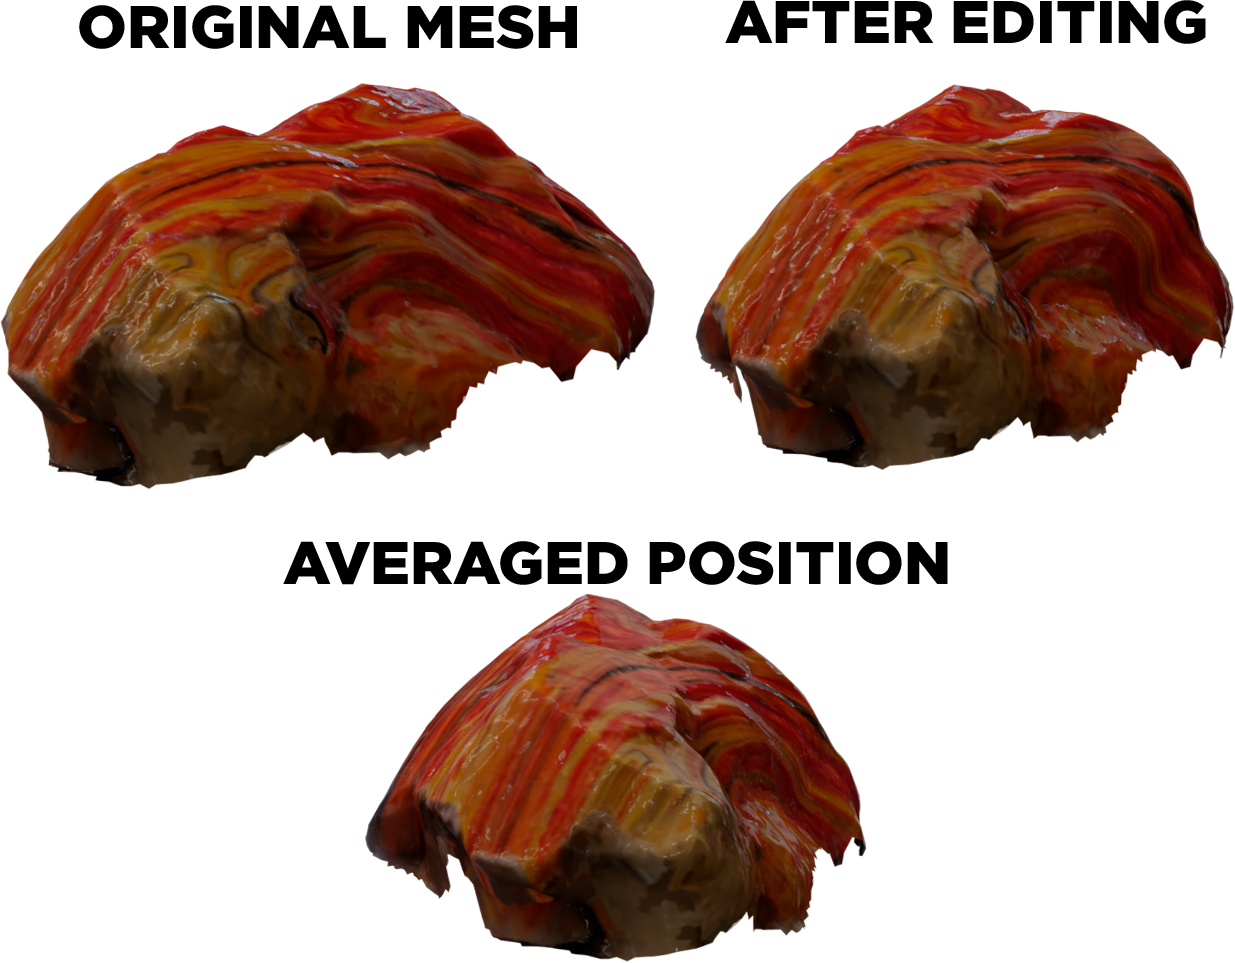
\includegraphics[width=35ex]{graphics/glassRock_three.png}
    \caption{The object used to test the average}
    \label{fig:glassRock_three}
\end{figure}

\section{Character}
\label{sec:characterPlaceholder}
The rigged character used for testing the optimisation is on figure \ref{fig:character_poses}. It was generated with the program MakeHuman™. It is animated for testing purposes, some poses of the animation are shown.

\begin{figure}[ht]
    \centering
    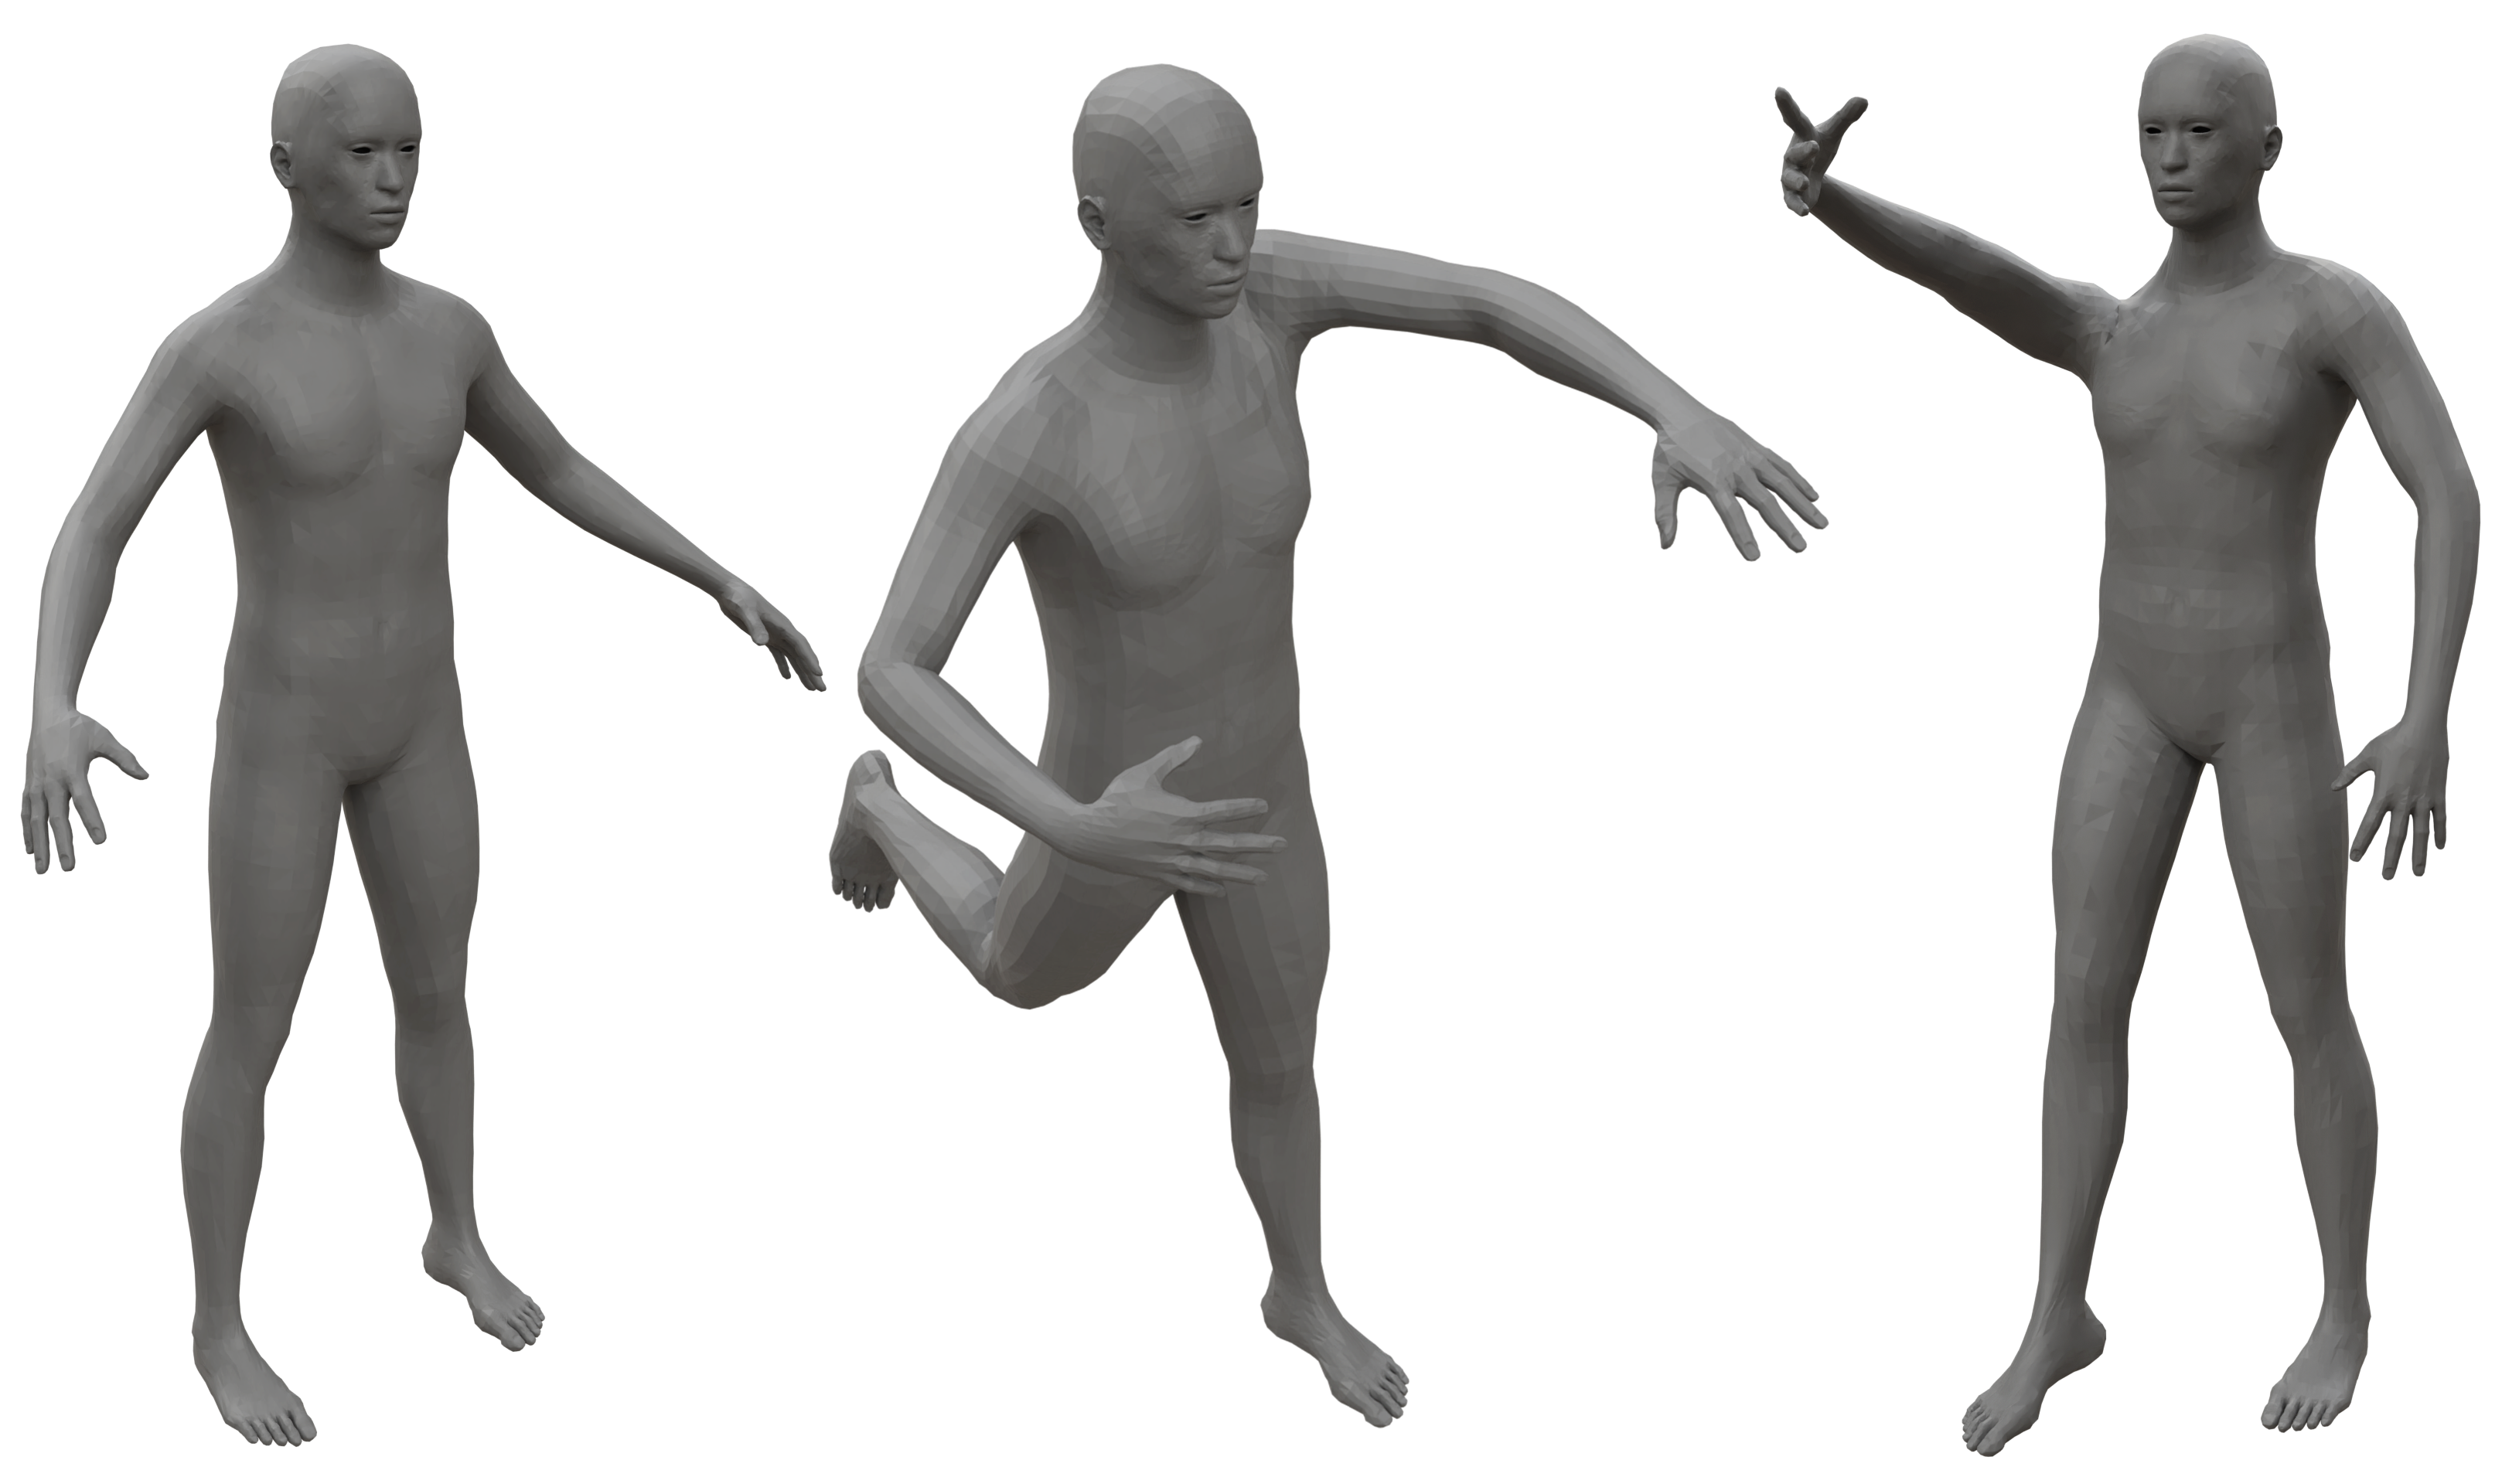
\includegraphics[width=\textwidth]{graphics/character_poses.png}
    \caption[The human model used for testing]{The human model used for testing, in rest pose (left) and in two poses}
    \label{fig:character_poses}
\end{figure}

\section{Desparsification}
\label{sec:despars_results}
Certain pictures of the the mesh showing how many bones influence each vertex: before (Figure \ref{fig:beforeDesparse}) and after (Figure \ref{fig:afterDesparse}) the desparsification algorithm. Red, a vertex is influenced by one bone; orange, by two bones; yellow, by three; green, by four bones (the desired amount); blue, by more than five bones.

Moreover, we now are going to show further images, with a single bone: the vertices that are influenced by this bone with weights $>0$ (green), the vertices that are influenced by it with weights equal to $0$ (yellow) and the vertices that are not influenced by it (blue) (Figures \ref{fig:pelvis_spine}, \ref{fig:arm_r}, \ref{fig:arm_l}).

\begin{figure}[hp]
    \centering
    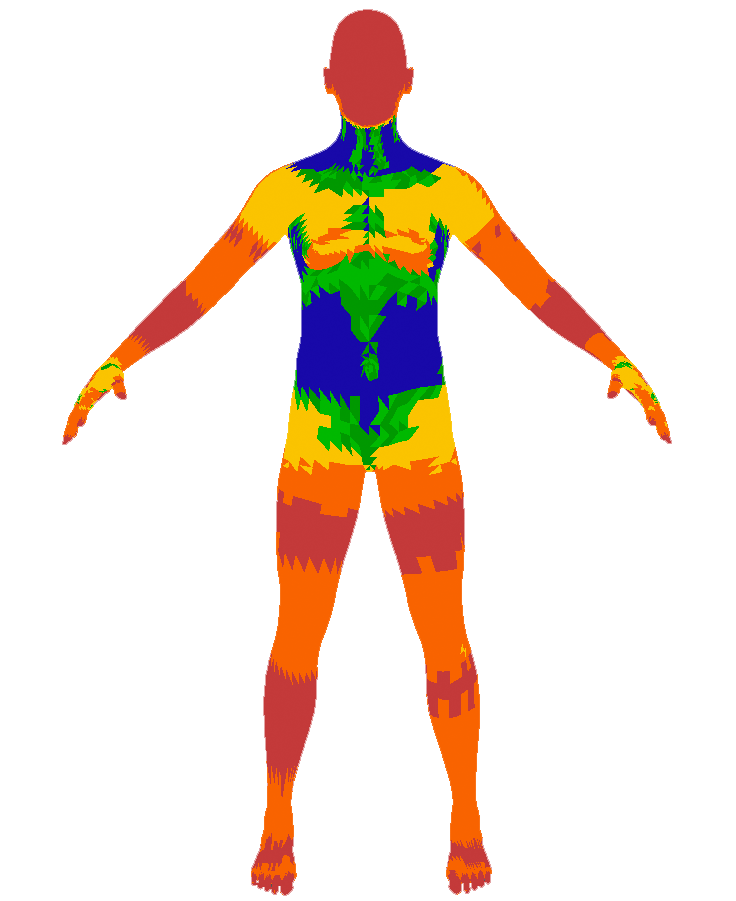
\includegraphics[width=50ex]{graphics/bfDesparse.png}
    \caption{Mesh before desparsification}
    \label{fig:beforeDesparse}
\end{figure}

\begin{figure}[hp]
\centering
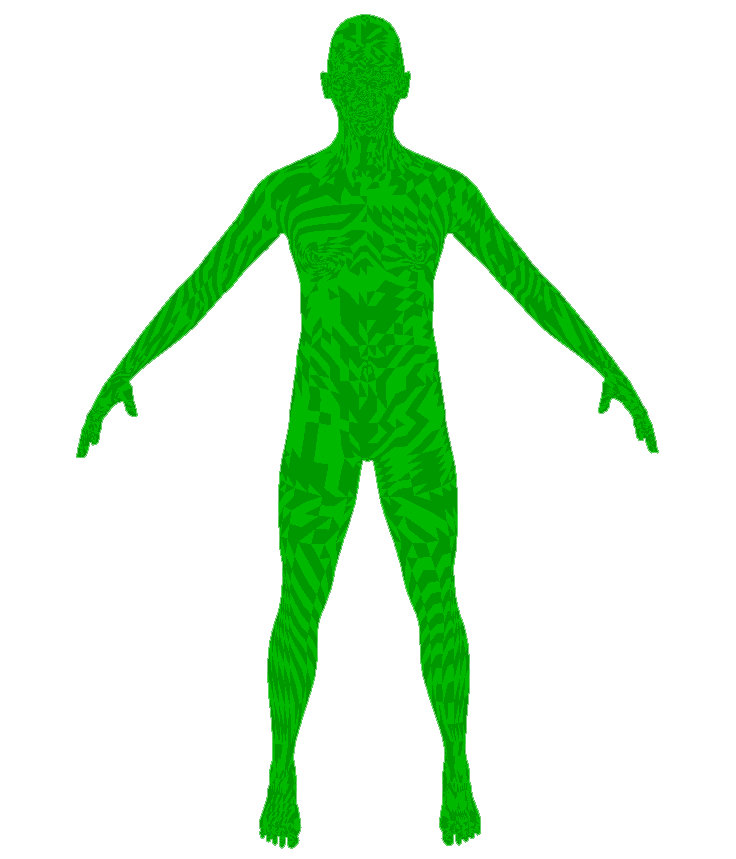
\includegraphics[width=50ex]{graphics/aftDesparse.png}
\caption{Mesh after desparsification}
\label{fig:afterDesparse}
\end{figure}

\newpage

\begin{figure}[hp]
\centering
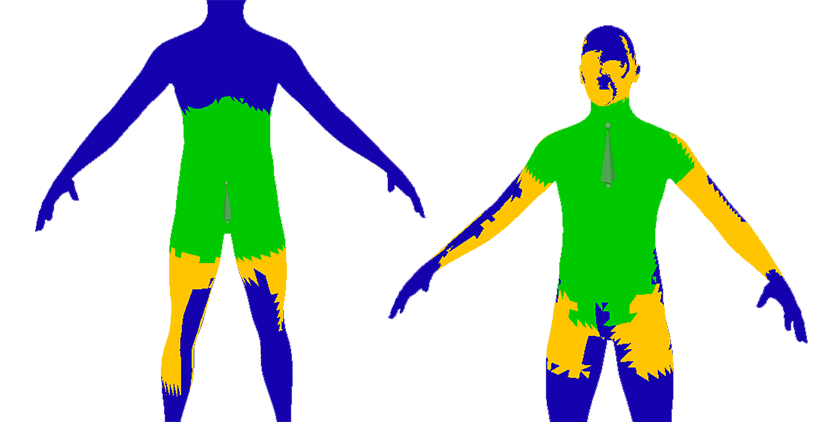
\includegraphics[width=50ex]{graphics/pelvis_spine.png}
\caption{Spine and pelvis after desparsification}
\label{fig:pelvis_spine}
\end{figure}

\begin{figure}[hp]
\centering
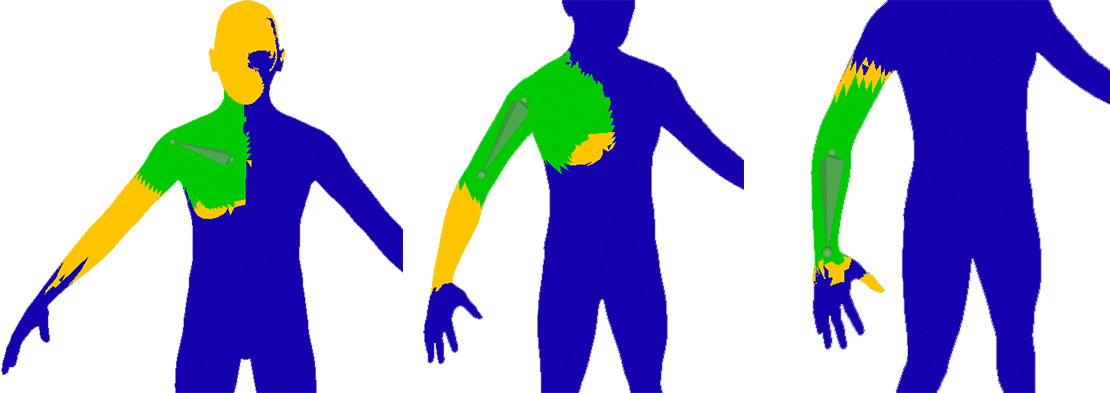
\includegraphics[width=50ex]{graphics/arm_r.png}
\caption{Right arm: clavicle, upper arm, lower arm}
\label{fig:arm_r}
\end{figure}

\begin{figure}[hp]
\centering
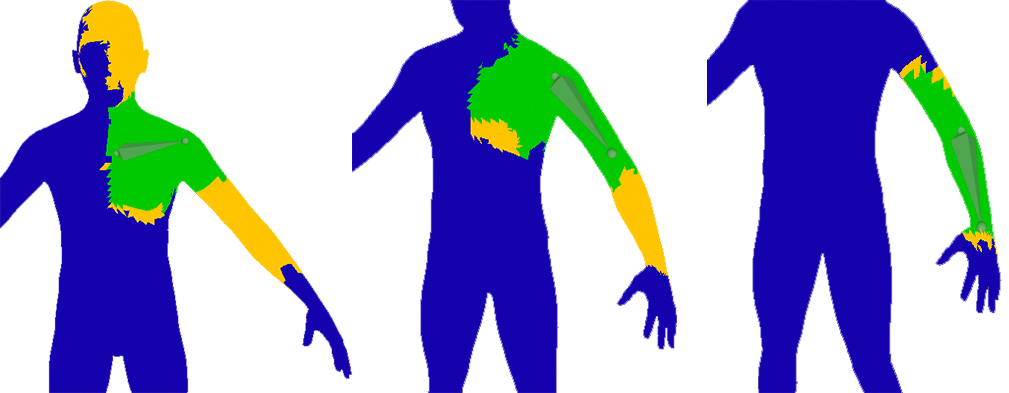
\includegraphics[width=46ex]{graphics/arm_l.png}
\caption{Left arm: clavicle, upper arm, lower arm}
\label{fig:arm_l}
\end{figure}

\section{Weights computation}
\label{sec:skinweightsolving_results}
Figures \ref{fig:result_forearm_l}, \ref{fig:result_forearm_l_2}, \ref{fig:result_upperarm_r} and \ref{fig:result_lowerarm_r} represent the four states of a posed mesh during animation sculpting. The user only sees the first and the last state.

Figure \ref{fig:optimisation_poses} represents the resulting vertex weights in a different pose than the edited one, in comparison to sculpting without the optimisation.

\begin{figure}[hp]
    \centering
    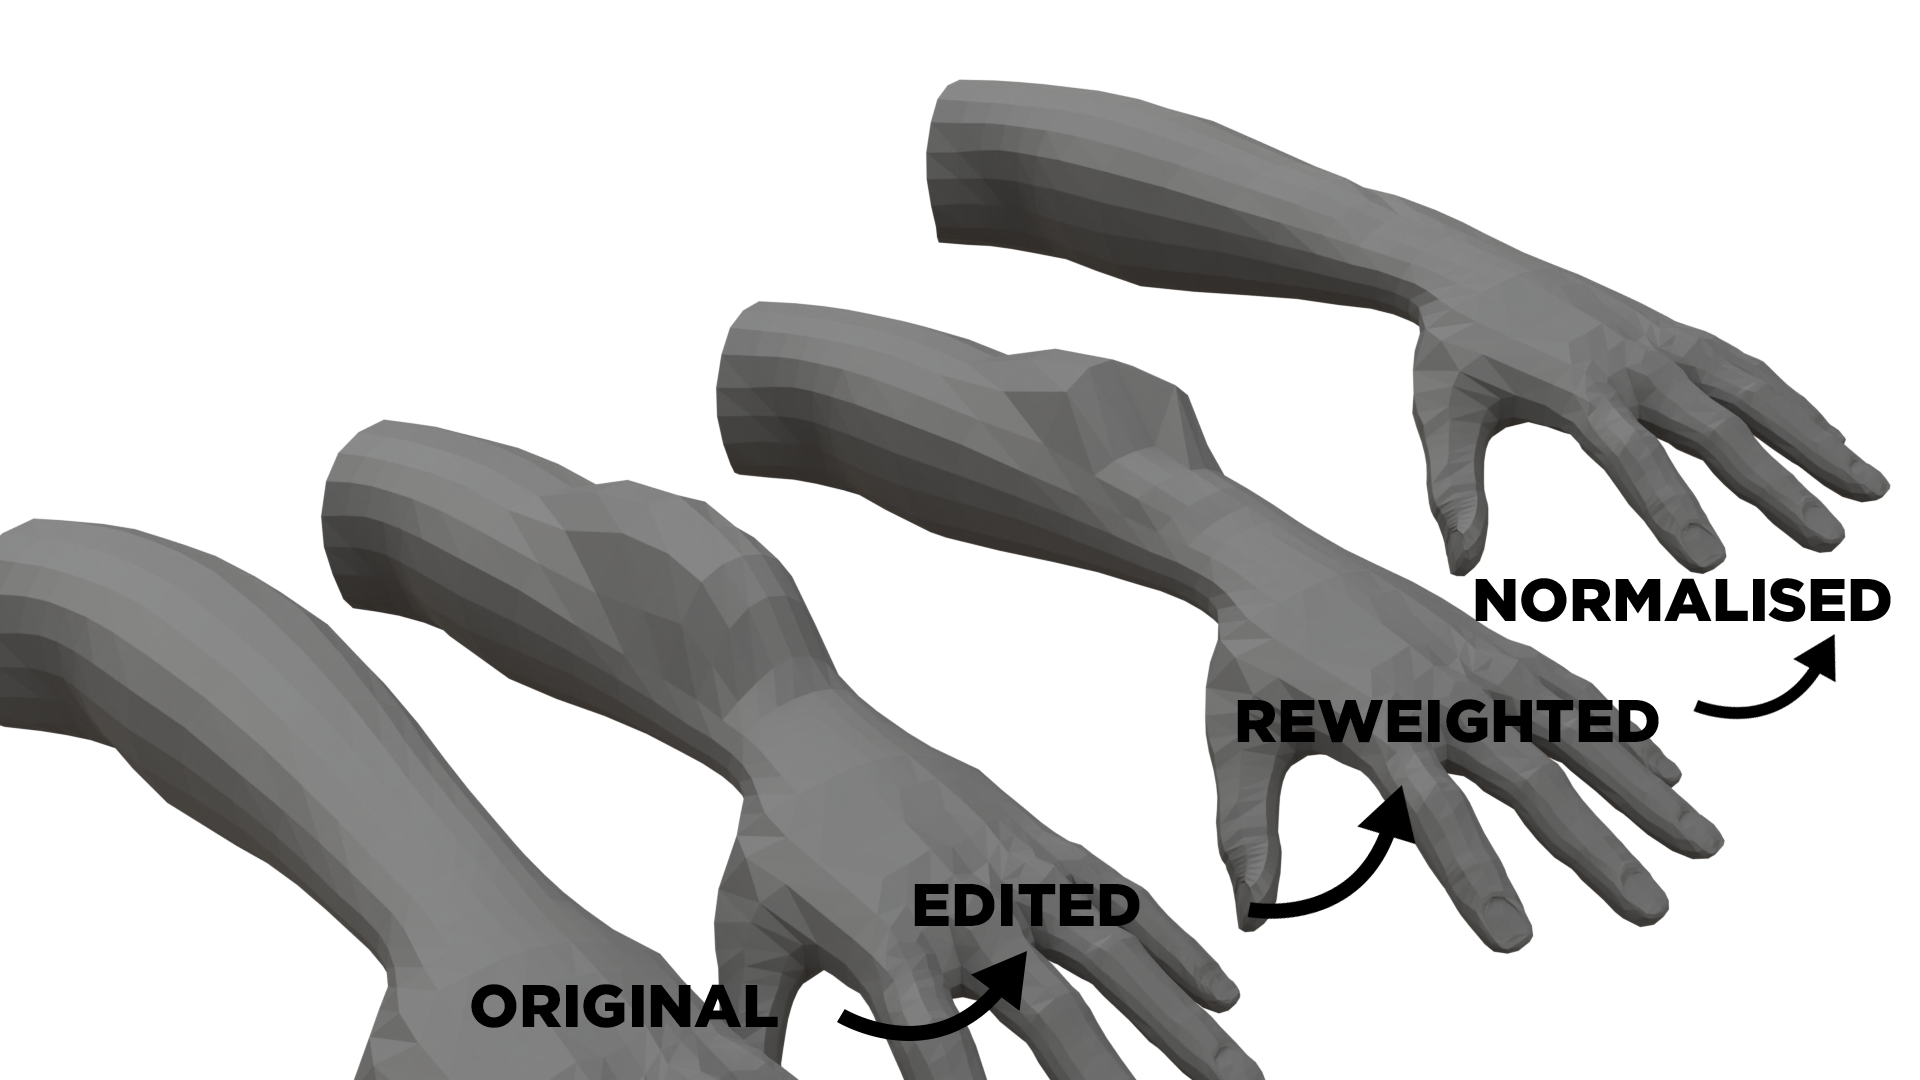
\includegraphics[width=65ex]{graphics/result_forearm_l.png}
    \caption{Left forearm, first attempt}
    \label{fig:result_forearm_l}
\end{figure}

\begin{figure}[hp]
    \centering
    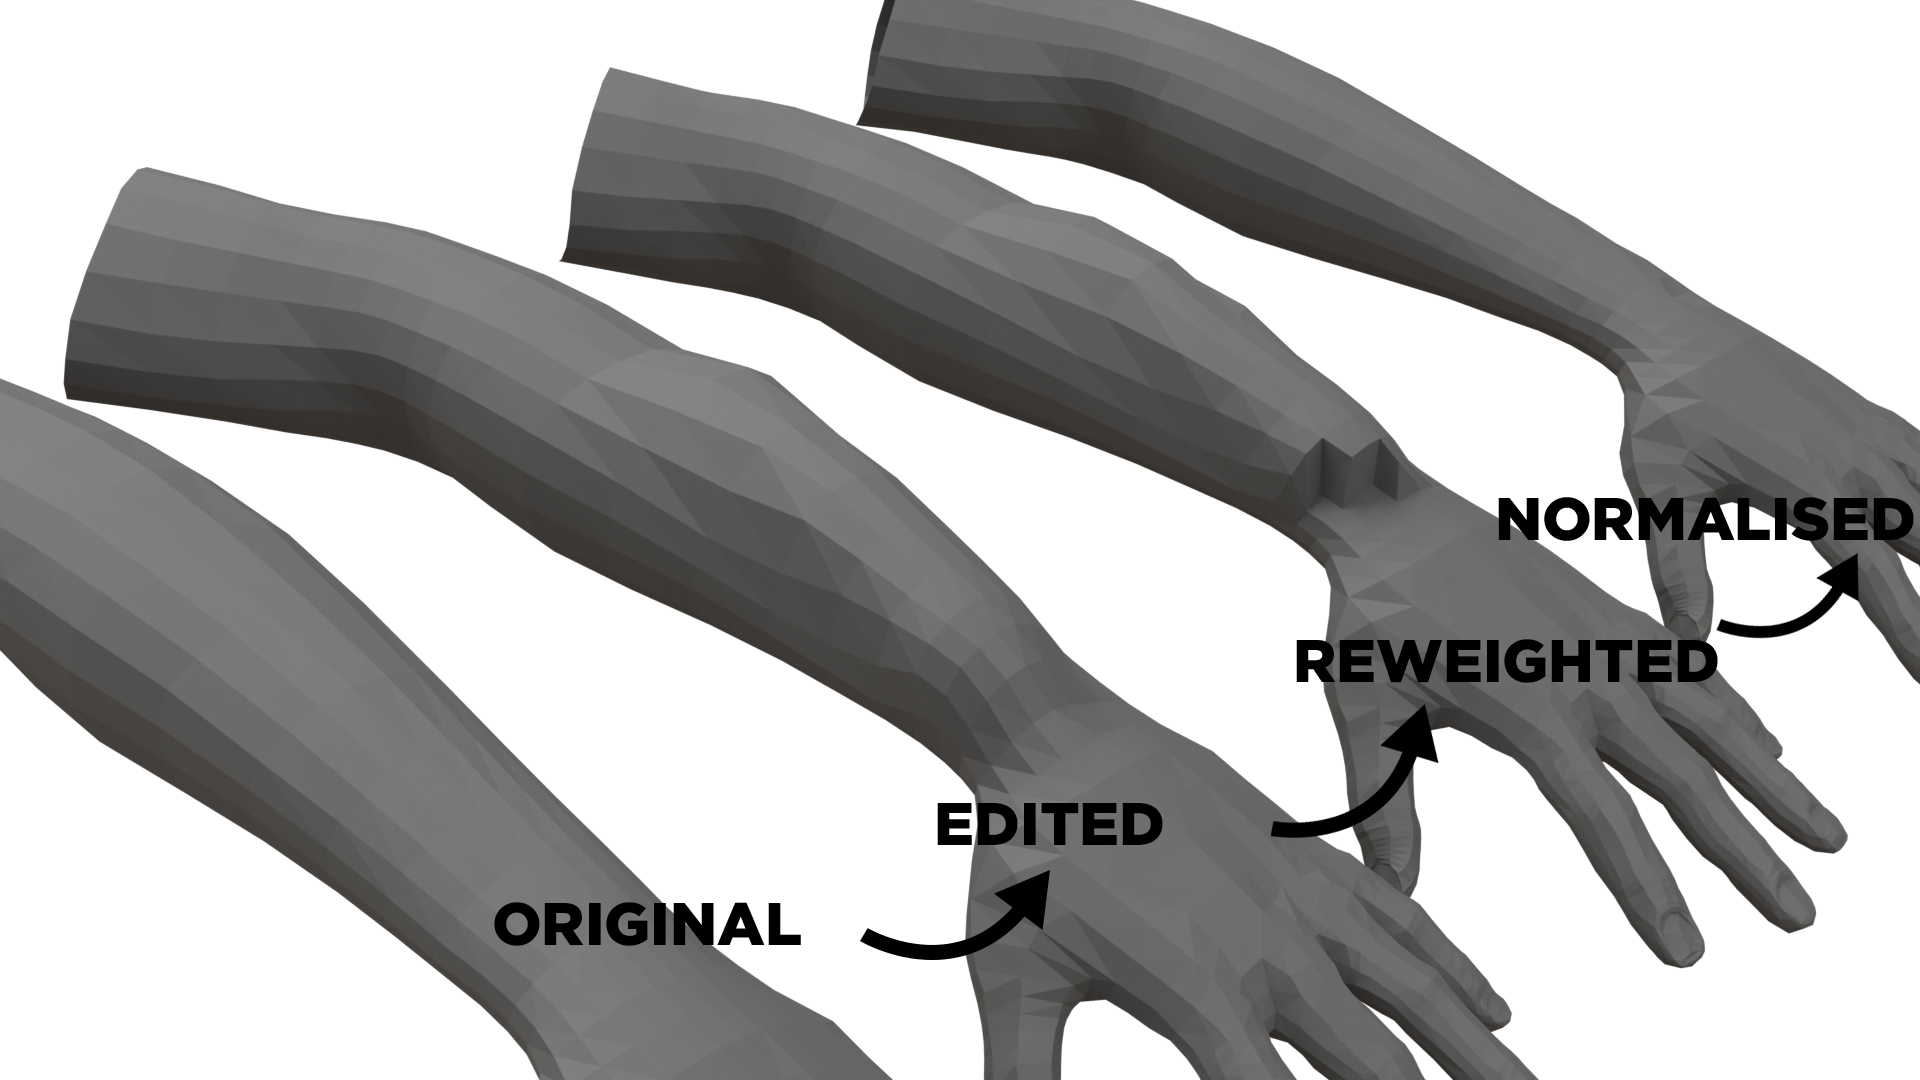
\includegraphics[width=65ex]{graphics/result_forearm_l_2.png}
    \caption{Left forearm, second attempt}
    \label{fig:result_forearm_l_2}
\end{figure}

\begin{figure}[hp]
    \centering
    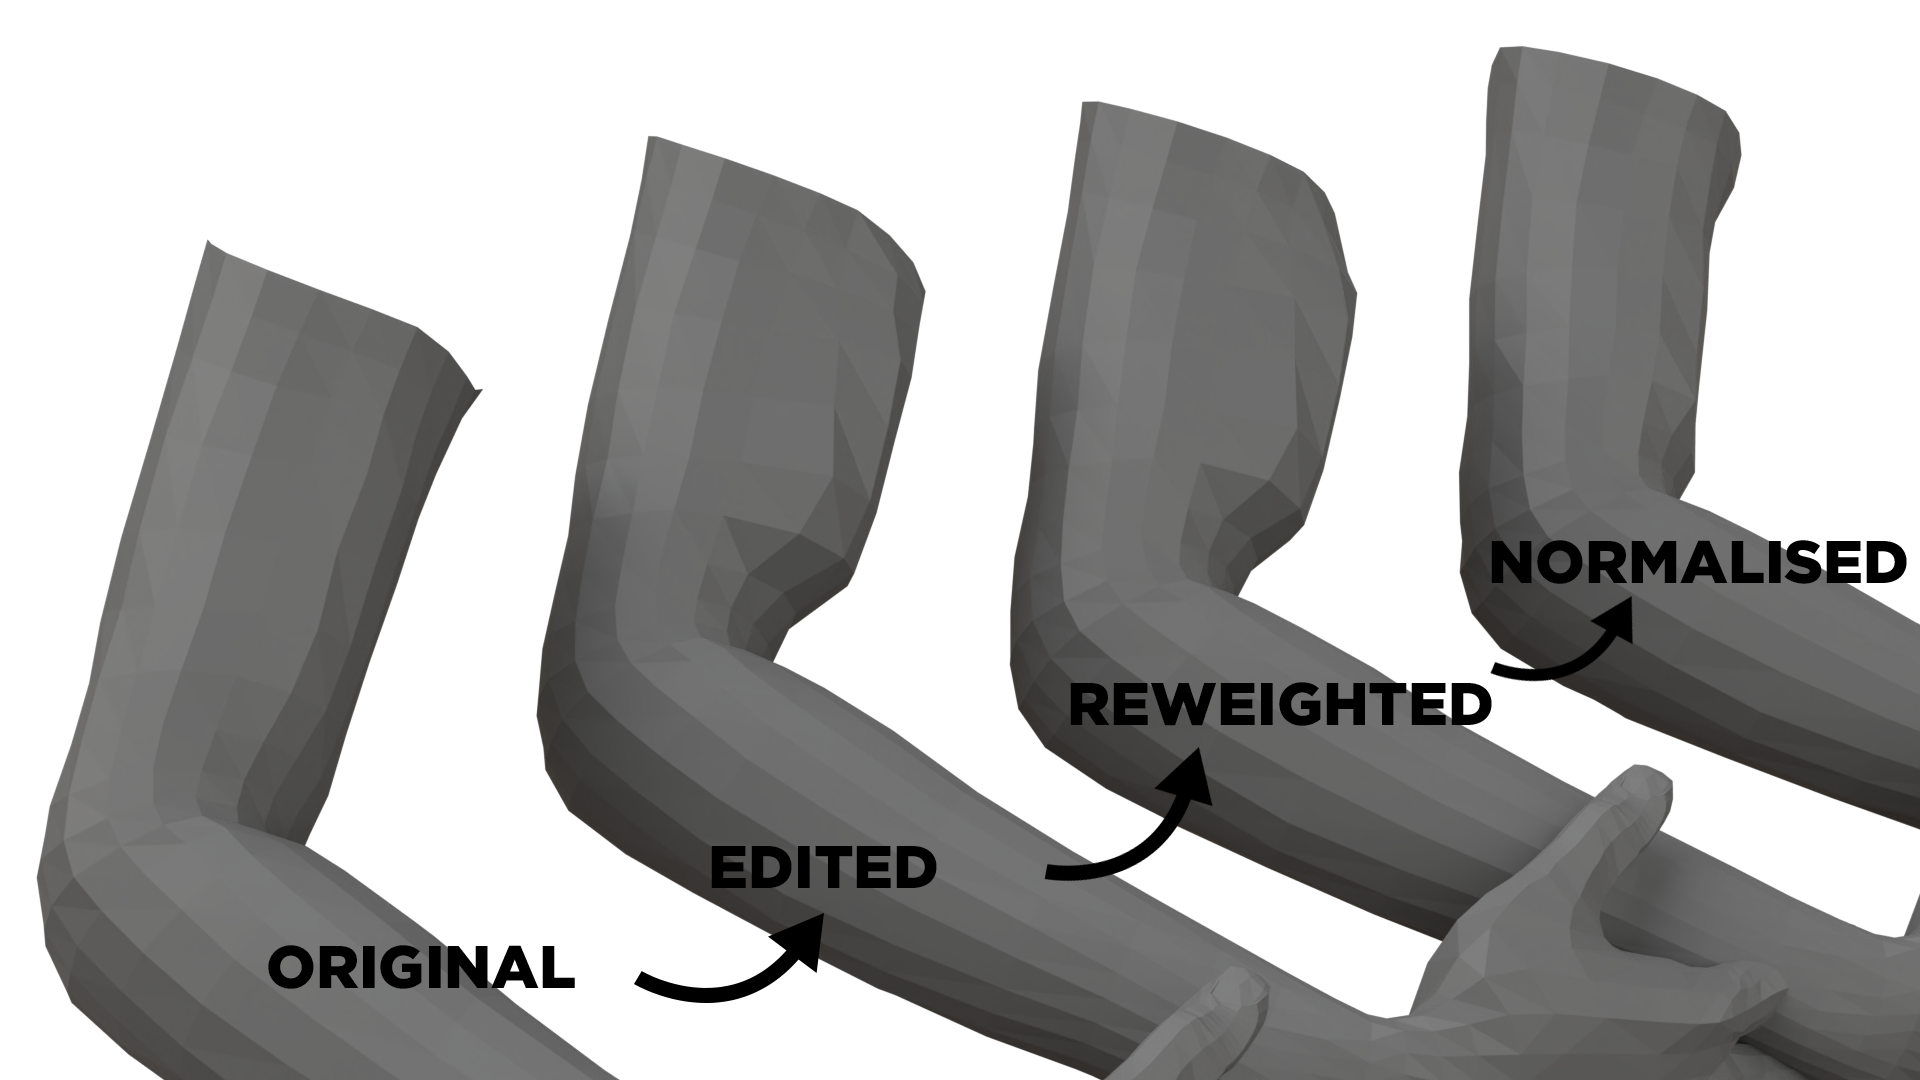
\includegraphics[width=65ex]{graphics/result_upperarm_r.png}
    \caption{Right upper arm}
    \label{fig:result_upperarm_r}
\end{figure}

\begin{figure}[hp]
    \centering
    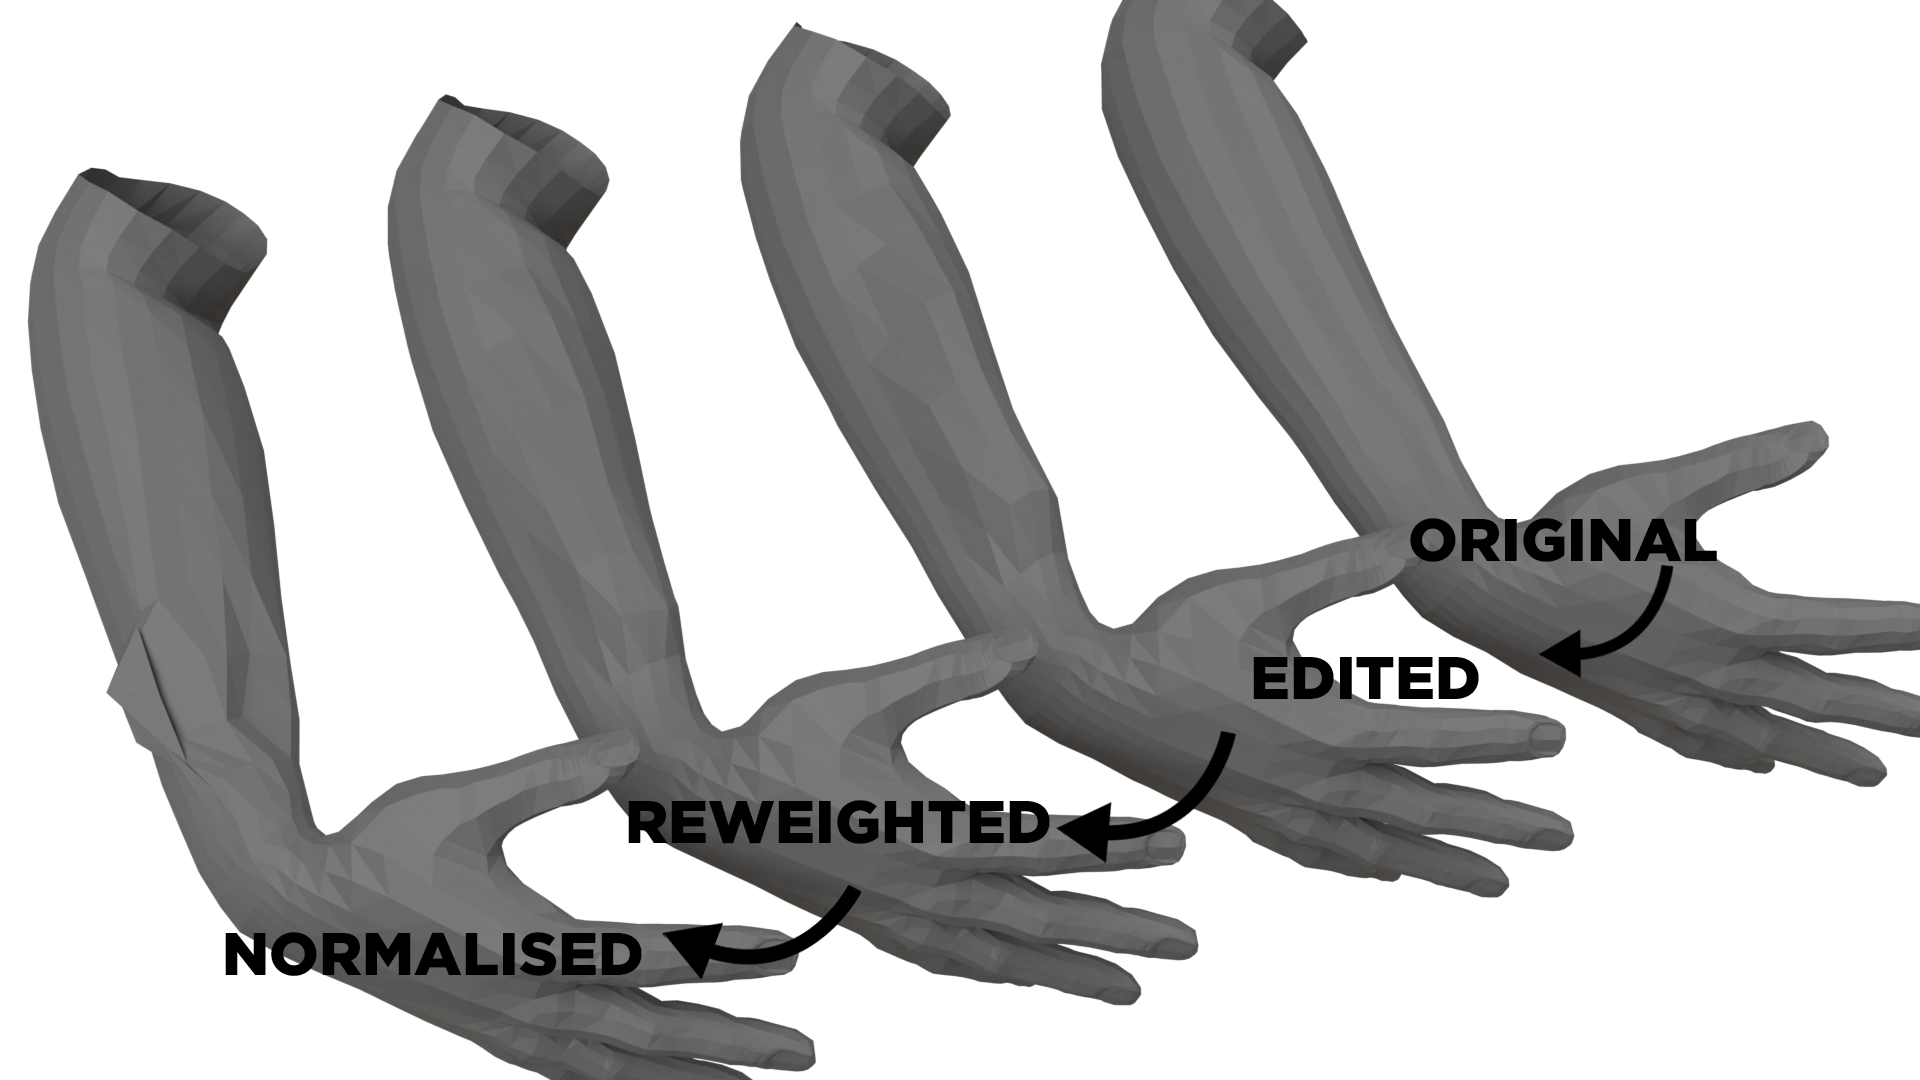
\includegraphics[width=65ex]{graphics/result_lowerarm_r.png}
    \caption{Right lower arm}
    \label{fig:result_lowerarm_r}
\end{figure}

\begin{figure}[hp]
    \centering
    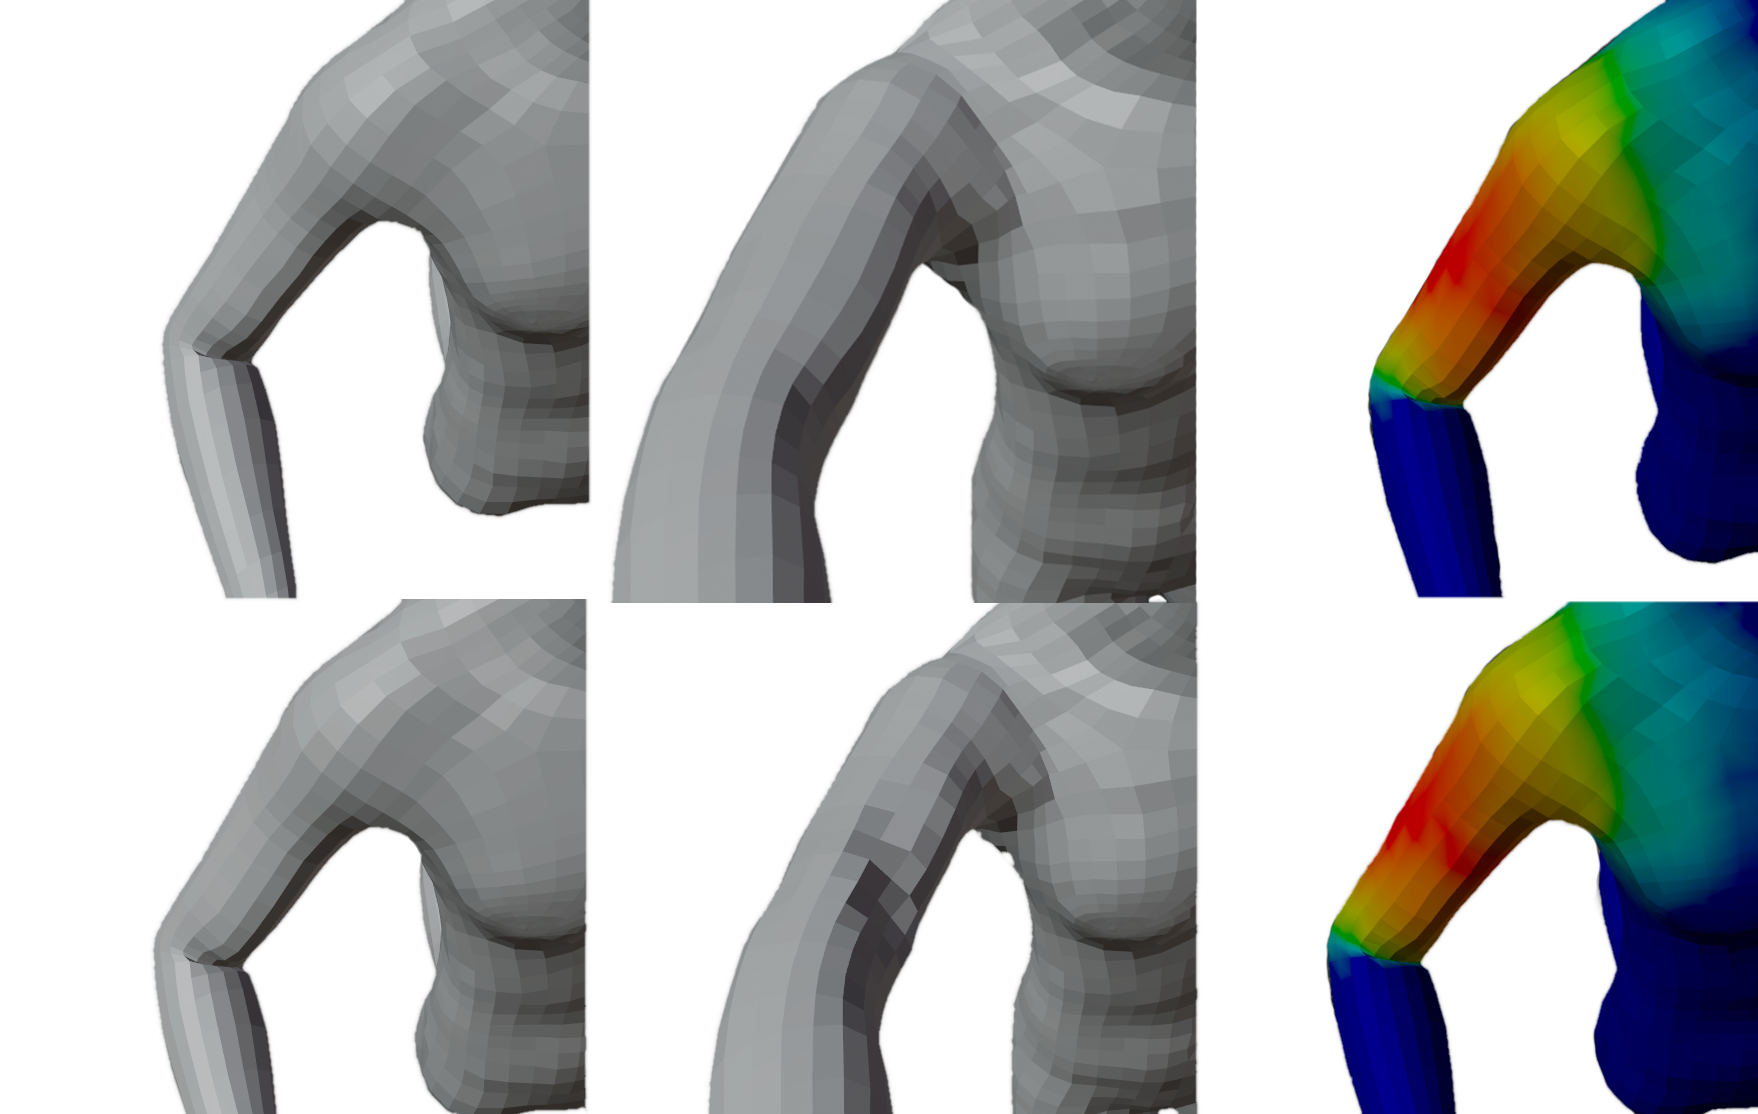
\includegraphics[width=\textwidth]{graphics/optimisation_poses.png}
    \caption[The right upper arm before and after editing]{The right upper arm before (top row) and after (bottom row) editing (including normalisation). The middle column is the pose that has not been edited.}
    \label{fig:optimisation_poses}
\end{figure}

\chapter{Conclusion and future work}

Now, we can finally summarise the conclusions of our research, highlighting at the same time certain hints for the future.

We have developed a plug-in: this, clearly, has some limitations. However, this prepares a good framework for any future development. Blender is definitely confirmed to be a platform ready to further experiment on our idea.

The optimising approach works correctly: it computes new weights close to the original editing. However, the re-calculated weights only work in the edited pose, most of the time; the other poses, on the other hand, result in a degenerated shape. This issue may be solved by evaluating weights based upon the ones coming from other poses.

Moreover, Blender only interpolates matrices with the (0;1) bounded range weights. The normalisation process we applied in order to bypass the issue, is not efficient enough. This may be due to a poor choice of new bone slots per vertex inside the desparsification algorithm; or due to our normalisation approach. That being so, it is possible to solve it by changing the desparsification algorithm or by using a solver that already implements said bounds.

Although we established that Blender is ready for the analysis of this project, we can scratch this idea and build an entire new framework that does not require any bound (see idea proposed in section \ref{sec:framework_from_scratch}). This would completely eliminate the necessity of normalising. However, it might compromise compatibility with other software. Therefore, said normalisation might be necessary after the optimisation is complete.

In conclusion, there is a limit in modifying just the weights after the optimisation. In fact, there is the possibility to have more degrees of freedom by also modifying the vertices positions in rest pose. This means, constructing a new system with more than three variables. The result of this new inverse problem might be more precise and less prone to errors.

\bibliographystyle{acm}
\bibliography{libs/bibliography}

\cleardoublepage

\end{document}